\documentclass [11pt,twoside]{article}
\usepackage[utf8]{inputenc}
\usepackage[T1]{fontenc}
\usepackage{listings}
\usepackage{color}
\usepackage{caption}
\usepackage{subcaption}

\definecolor{dkgreen}{rgb}{0,0.6,0}
\definecolor{secblue}{rgb}{0.3,0.6,0.7}
\definecolor{bluesec}{rgb}{0.3,0.6,0.7}
\definecolor{secred}{rgb}{0.7,0.3,0.3}

%Page margins, header and footer positions
\usepackage{geometry}
 \geometry{
 a4paper,
 total={210mm,297mm},
 left=25mm,
 right=25mm,
 top=30mm,
 bottom=25mm,
 headsep=7mm}

\interfootnotelinepenalty=10000

%To display filling dots in the TOC for all entries
\usepackage[titles]{tocloft}
\renewcommand{\cftsecleader}{\cftdotfill{\cftdotsep}}

%Define new header and footer style
\usepackage{fancyhdr}

\pagestyle{fancy}
\fancyhf{}
\lhead{\color{Gray}{\small{TrackMe project by Leonardo Barilani, William Bonvini, Lorenzo Carnaghi}}}
\lfoot{\textcolor{Gray}{\small{Copyright © 2018, Leonardo Barilani, William Bonvini, Lorenzo Carnaghi – All rights reserved}}}
\rfoot{\textcolor{Gray}{\thepage}}
\renewcommand{\headrulewidth}{0pt}

%PACKAGES
\usepackage{wasysym}
\usepackage{pifont}

\newcommand{\supported}{\ding{52}\xspace}
\newcommand{\unsupported}{\ding{55}\xspace}
\newcommand{\partsupported}{\textcolor{black!40}{\ding{52}}\xspace}
\newcommand{\lowsupported}{\textcolor{black!20}{\ding{52}}\xspace}
\newcommand{\unknowsupported}{\textbf{?}\xspace}

%Font: Times
\usepackage{times}
%Change monospaced font
\renewcommand{\ttdefault}{lmtt}

%tables
\usepackage{tabu}
\usepackage{tabularx}
\usepackage{ltablex}
\usepackage{longtable}
\usepackage{float} % To allow the use of H modifier in long tables

%landscape mode
\usepackage{pdflscape}
\usepackage{rotating}
\usepackage{caption}

%make landscape mode be sensitive to even and odd pages
%start
\def\myrotate{\ifodd\c@page\else-\fi 90}
\makeatletter
\global\let\orig@begin@landscape=\landscape%
\global\let\orig@end@landscape=\endlandscape%
\gdef\@true{1}
\gdef\@false{0}
\gdef\landscape{%
    \global\let\within@landscape=\@true%
    \orig@begin@landscape%
}%
\gdef\endlandscape{%
    \orig@end@landscape%
    \global\let\within@landscape=\@false%
}%
\@ifpackageloaded{pdflscape}{%
    \gdef\pdf@landscape@rotate{\PLS@Rotate}%
}{
    \gdef\pdf@landscape@rotate#1{}%
}
\let\latex@outputpage\@outputpage
\def\@outputpage{
    \ifx\within@landscape\@true%
        \if@twoside%
            \ifodd\c@page%
                \gdef\LS@rot{\setbox\@outputbox\vbox{%
                    \pdf@landscape@rotate{-90}%
                    \hbox{\rotatebox{90}{\hbox{\rotatebox{180}{\box\@outputbox}}}}}%
                }%
            \else%
                \gdef\LS@rot{\setbox\@outputbox\vbox{%
                    \pdf@landscape@rotate{+90}%
                    \hbox{\rotatebox{90}{\hbox{\rotatebox{0}{\box\@outputbox}}}}}%
                }%
            \fi%
        \else%
            \gdef\LS@rot{\setbox\@outputbox\vbox{%
                \pdf@landscape@rotate{+90}%
                \hbox{\rotatebox{90}{\hbox{\rotatebox{0}{\box\@outputbox}}}}}%
            }%
        \fi%
    \fi%
    \latex@outputpage%
}
\makeatother
%end

%graphics
\usepackage{graphicx}
\usepackage[dvipsnames, table]{xcolor}
%If you upload images from PC, you need to insert code for the path here (different for Windows and Unix OS)

%References
%\usepackage{xpatch}
%\usepackage[backend=biber, style=numeric, citestyle=numeric, sorting=none]{biblatex}
%\addbibresource{main.bib}

%Other
\usepackage{ifthen}
\usepackage{xspace}
\usepackage{enumitem}
\usepackage{amssymb}
\usepackage[pdftex, colorlinks]{hyperref}
\newcommand{\comment}[1]{{\color{Red}$\blacktriangleright$ Comment: #1 $\blacktriangleleft$}}


% Some utilities\ldots
\usepackage{soul}
\usepackage{tikz}

\usetikzlibrary{calc}
\usetikzlibrary{decorations.pathmorphing}


\makeatletter

\newcommand{\defhighlighter}[3][]{%
  \tikzset{every highlighter/.style={color=#2, fill opacity=#3, #1}}%
}

\defhighlighter{yellow}{.5}

\newcommand{\highlight@DoHighlight}{
  \fill [ decoration = {random steps, amplitude=1pt, segment length=15pt}
        , outer sep = -15pt, inner sep = 0pt, decorate
       , every highlighter, this highlighter ]
        ($(begin highlight)+(0,8pt)$) rectangle ($(end highlight)+(0,-3pt)$) ;
}

\newcommand{\highlight@BeginHighlight}{
  \coordinate (begin highlight) at (0,0) ;
}

\newcommand{\highlight@EndHighlight}{
  \coordinate (end highlight) at (0,0) ;
}

\newdimen\highlight@previous
\newdimen\highlight@current

\DeclareRobustCommand*\highlight[1][]{%
  \tikzset{this highlighter/.style={#1}}%
  \SOUL@setup
  %
  \def\SOUL@preamble{%
    \begin{tikzpicture}[overlay, remember picture]
      \highlight@BeginHighlight
      \highlight@EndHighlight
    \end{tikzpicture}%
  }%
  %
  \def\SOUL@postamble{%
    \begin{tikzpicture}[overlay, remember picture]
      \highlight@EndHighlight
      \highlight@DoHighlight
    \end{tikzpicture}%
  }%
  %
  \def\SOUL@everyhyphen{%
    \discretionary{%
      \SOUL@setkern\SOUL@hyphkern
      \SOUL@sethyphenchar
      \tikz[overlay, remember picture] \highlight@EndHighlight ;%
    }{%
    }{%
      \SOUL@setkern\SOUL@charkern
    }%
  }%
  %
  \def\SOUL@everyexhyphen##1{%
    \SOUL@setkern\SOUL@hyphkern
    \hbox{##1}%
    \discretionary{%
      \tikz[overlay, remember picture] \highlight@EndHighlight ;%
    }{%
    }{%
      \SOUL@setkern\SOUL@charkern
    }%
  }%
  %
  \def\SOUL@everysyllable{%
    \begin{tikzpicture}[overlay, remember picture]
      \path let \p0 = (begin highlight), \p1 = (0,0) in \pgfextra
        \global\highlight@previous=\y0
        \global\highlight@current =\y1
      \endpgfextra (0,0) ;
      \ifdim\highlight@current < \highlight@previous
        \highlight@DoHighlight
        \highlight@BeginHighlight
      \fi
    \end{tikzpicture}%
    \the\SOUL@syllable
    \tikz[overlay, remember picture] \highlight@EndHighlight ;%
  }%
  \SOUL@
}

\makeatother

% Common abbrev. are set as commands to ensure proper spacing after the dot
\RequirePackage{xspace}
\newcommand{\ie}{i.e.\@\xspace}
\newcommand{\aka}{a.k.a.\@\xspace}
\newcommand{\Ie}{I.e.\@\xspace}
\newcommand{\cf}{cf.\@\xspace}
\newcommand{\Cf}{Cf.\@\xspace}
\newcommand{\eg}{e.g.\@\xspace}
\newcommand{\Eg}{E.g.\@\xspace}
\newcommand{\etal}{et al.\@\xspace}
\newcommand{\etc}{etc.\@\xspace}
\newcommand{\wrt}{w.r.t.\@\xspace}
\newcommand{\Wrt}{W.r.t.\@\xspace}



\date{}


\begin{document}

%TITLE PAGE

\begin{titlepage}


%LOGO

{\begin{table}[t!]
\centering
\begin{tabu} to \textwidth { X[1.3,r,p] X[1.7,l,p] }
\textcolor{Blue}
{\textbf{\small{TrackMe project L. Barilani, W. Bonvini, L. Carnaghi}}} & 
\includegraphics[scale=0.5]{Images/PolimiLogo}
\end{tabu}
\end{table}}~\\ [7cm]

%TITLE 

\begin{flushleft}

%Replace the text string with your title
{\textcolor{Blue}{\textbf{\Huge{Requirement Analysis and Specification
        Document}}}} \\ [1cm]

\end{flushleft}

\end{titlepage}

%Define deliverable specific info
%Replace cell contents where needed
\begin{table}[h!]
\begin{tabu} to \textwidth { X[0.3,r,p] X[0.7,l,p] }
\hline

\textbf{Deliverable:} & RASD\\
\textbf{Title:} & Requirement Analysis and Verification Document \\
\textbf{Authors:} & Leonardo Barilani, William Bonvini, Lorenzo Carnaghi \\
\textbf{Version:} & 1.0 \\ 
\textbf{Date:} & 8-November-2018 \\
\textbf{Download page:} & https://github.com/Lockyard/BarilaniBonviniCarnaghi \\
\textbf{Copyright:} & Copyright © 2018, Leonardo Barilani, William Bonvini, Lorenzo Carnaghi – All rights reserved \\
\hline
\end{tabu}
\end{table}




\setcounter{page}{2}



%------------------------------------------------------------------------------------------------------------------------------------------------
\newpage
\color{secred}
{\color{secred}\addcontentsline{toc}{section}{Table of Contents}}
\tableofcontents
\color{black}

%------------------------------------------------------------------------------------------------------------------------------------------------
\clearpage
{\color{secblue}{\section{Introduction}}}
\label{sect:introduction}
\color{black}
{\color{secblue}\subsection{Purpose}} The purpose of this document is to give an overview of the Data4Help, AutomatedSOS and Track4Run services, and specify its requirements, functional and non functional and associated technical constraints.
People who are interested in this service would need to download the relative app on their smartphone, and their data will be automatically collected by TrackMe.
Data4Help is a service which aims to gather information about people's health status in order to share it with third-parties.
AutomatedSOS aims to help ederly people by constantly monitoring their health status and automatically calling an ambulance in case of an emergency.
Track4Run's purpose is to organize races among runners. It allows the creation of a run and its enrollment. Also, it provides a real-time map of the runners for the spectators.

{\color{secblue}\subsubsection{Goals}}
\begin{itemize}
\item G1 - The Data4Help application gives constantly new data accordingly to users' activities.
\item G2 - Registered TPs (Third Parties) can send requests to specific users if they know their SSN or CF in order to retrieve specific data. These users can accept or refuse the proposal.
\item G3 - Registered TPs have access to make queries to Data4Help's database in order to get anonymized data by filtering by one or more parameters as they need.
\item G4 - Results for TPs' queries are given only if the number of matches is greater or equal than 1000.
\item G5 - Each user of the services offered by TrackMe is identifiable within the system in order to gather his data and communicate with him.
\item G6 - AutomatedSOS sends automatically an ambulance request when and only when user's values are below a specific critical threshold, specifying the user's position.
\item G7 - Users of Track4Run are able to create a run defining the precise path.
\item G8 - Users of Track4Run are able to take part in a created run as runners.
\item G9 - Users of Track4Run can see real-time runners' positions in runs such runners are subscribed in.
\end{itemize}
{\color{secblue}\subsection{Scope}}
{\color{secblue}\subsubsection{Project description}}
Data4Help is a service mainly thought for big companies who want to make better targeted choices for their business. Since the service acquires the health status of the users, most of the companies interested in the service are supposely going to be related to lifestyle, fitness, and generally the sports field.
The position of the users could be a very useful information for third parties related to the transportation system and tourism.
Health status and position combined offer a good overview of the health situation of a population of a specific area selected by the third party. Such data can be used for pools and statistical purposes, so being attractive to health related realities: pharmacheutical industry, health organizations (state entities and non state ones).
The final product will consist in 3 main softwares:
\begin{itemize}
\item The server-side software;
\item The mobile application for standard-users;
\item The desktop application for third-parties users.
\end{itemize}
There are quite a few shared phenomena that occur in the projects:
\begin{itemize}
\item A third party requests a query in Data4Help;
\item One of the three apps gathers information;
\item AutomatedSOS calls an ambulance in case of an emergency;
\item A run gets created in Track4Run by an user.
\end{itemize}
{\color{secblue}\subsection{Definitions, Acronyms, Abbreviations}}
{\color{secblue}\subsubsection{Definitions}}
\begin{itemize}
\item User: a user is a person who uses at least one of Track4Run's services by installing it on its smartphone/PC and signing up.
\item Third-party: any organization/company/authority who registers to Data4Help in order to gather user's information.
\item Query: A filtered search asked to the Data4Help's DB.
\item Run: an event organized through Track4Run service, in a specific location.
\end{itemize}
{\color{secblue}\subsubsection{Acronyms}}
\begin{itemize}
\item \b{TP:} Third Party (TPs for plural)
\item \b{SSN:} Social Security Number
\item \b{CF:} Codice Fiscale
\item \b{DB:} Database
\item \b{ASOS:} AutomatedSOS
\end{itemize}
{\color{secblue}\subsubsection{Abbreviations}}
\begin{itemize}
\item \b{[Gx]:} x-th Goal
\item \b{[Dx]:} x-th Domain assumption
\item \b{[Rx]:} x-th Requirement
\item \b{[FRx]:} x-th Functional Requirement
\end{itemize}
{\color{secblue}\subsection{Revision history}}
the version 2 of the RASD present the following changes:
\begin{itemize}
\item removed chat system reference in mockups and use cases
\item Fixed english mistakes and typos
\item Modified Alloy model for Track4Run: It no more shows users subscribed as participants or spectators but instead there is a new information on which participants are visible in a certain time. The predicates and assertions partially changed, to show a more coherent aspect.
\item Added Data4Help's Third party's mockups 
\item Added the class TrackMe in the UML diagram
\end{itemize}

%------------------------------------------------------------------------------------------------------------------------------------------------
\clearpage
{\color{secblue}{\section{Overall Description}}}
\label{sect:overall}
\color{black}
{\color{secblue}\subsection{Product perspective}}
The following class diagram sums up conceptually the system behind the services Data4Help, AutomatedSOS and Track4Run.
\begin{figure}[H]
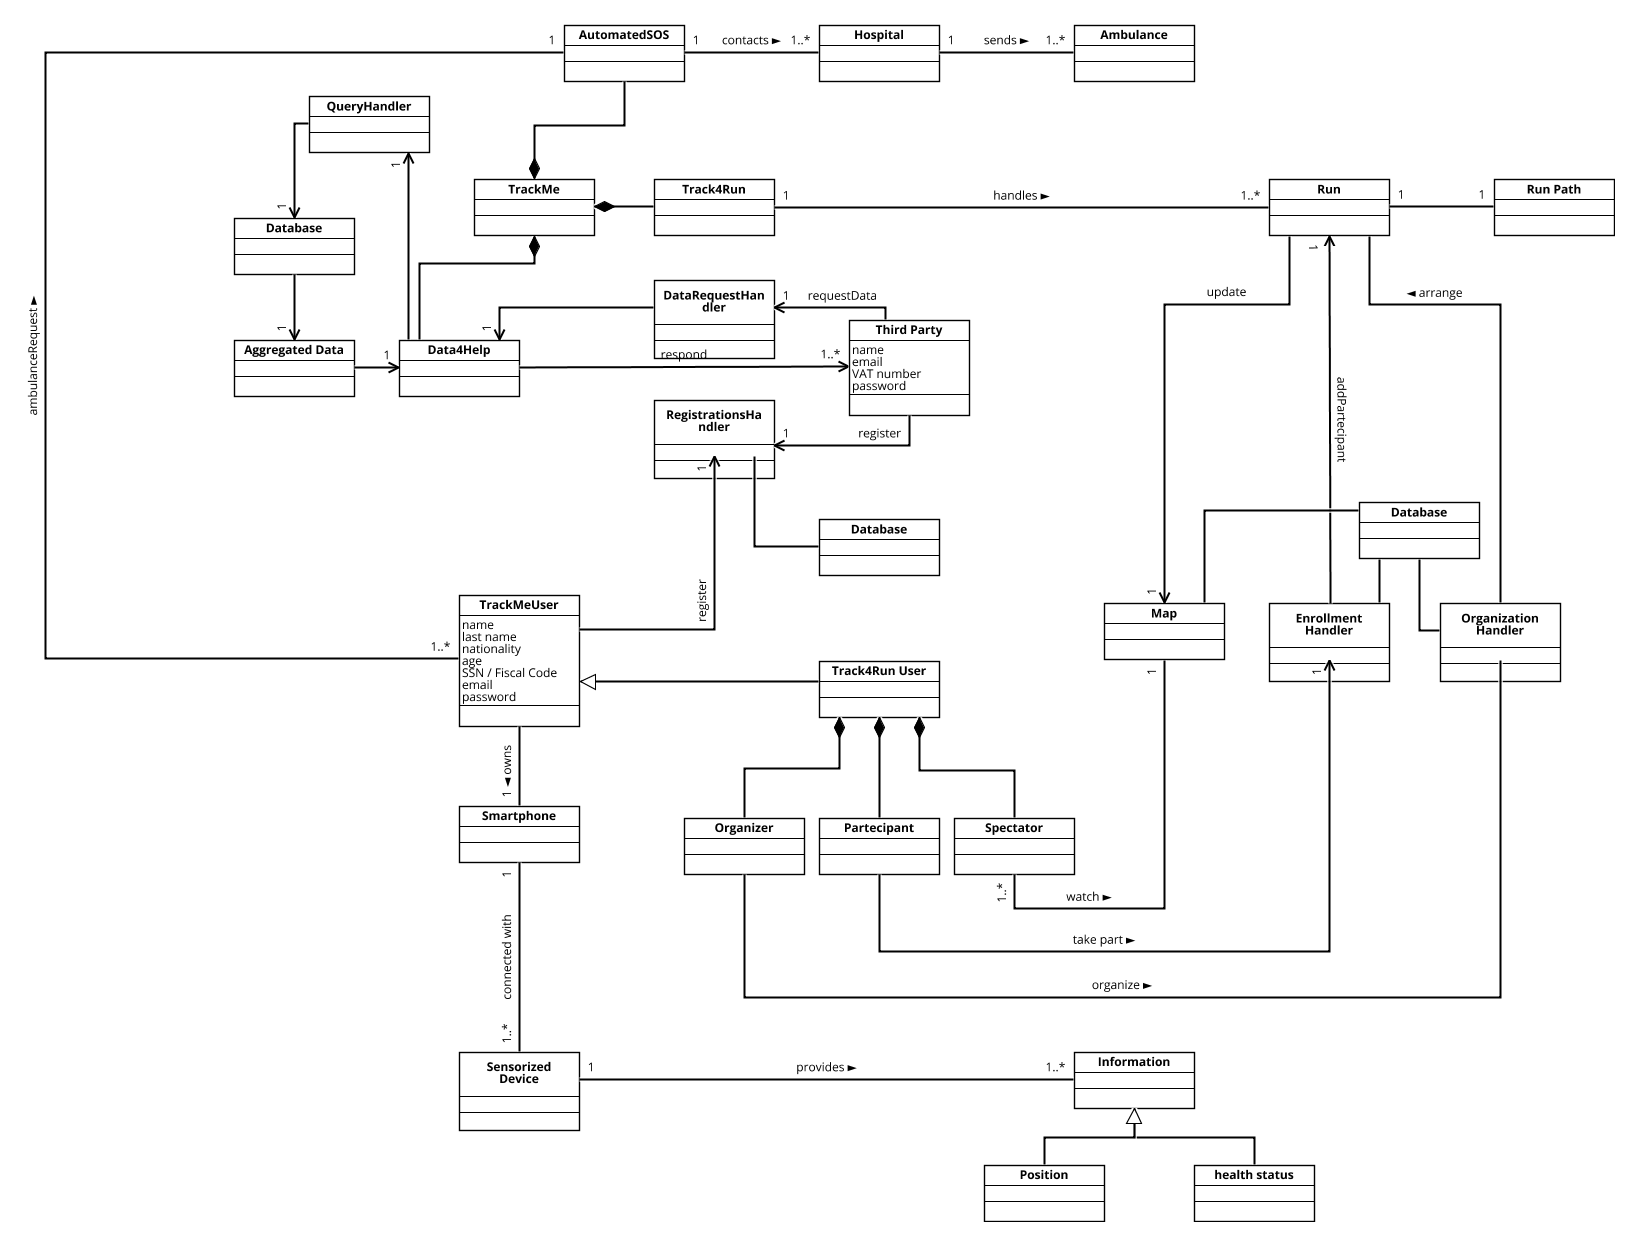
\includegraphics[width=\linewidth]{./Images/RASD_UML.png}
\centering
\caption{UML diagram}
\end{figure}
From this diagram it's visible that for the three services only one TrackMe account is needed to be created.
The class TrackMe is mainly a container of the three services.
Database is only one class, it gets repetead more than once only to make the diagram clearer to be looked at.

\newpage
Here will follow the state diagrams of each of the services provided by TrackMe.

\begin{figure}[H]
    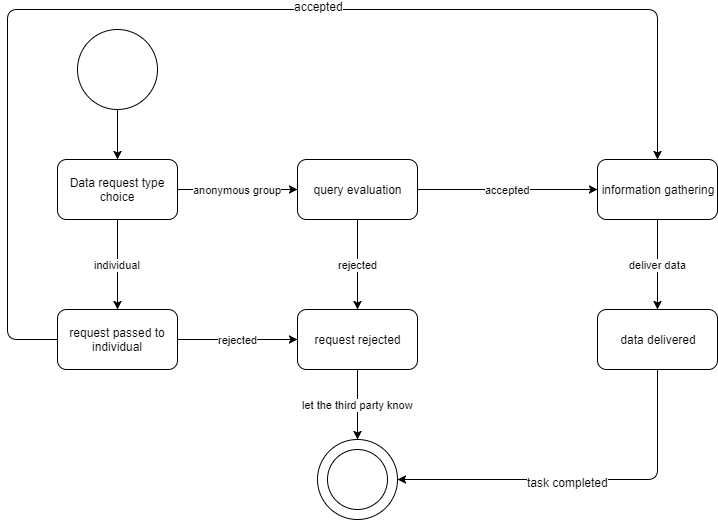
\includegraphics[width=\linewidth]{./Images/RASD_State_Diagram.png}
    \centering
    \caption{Data4Help state diagram}
  \end{figure}
  
  
  \begin{figure}[H]
    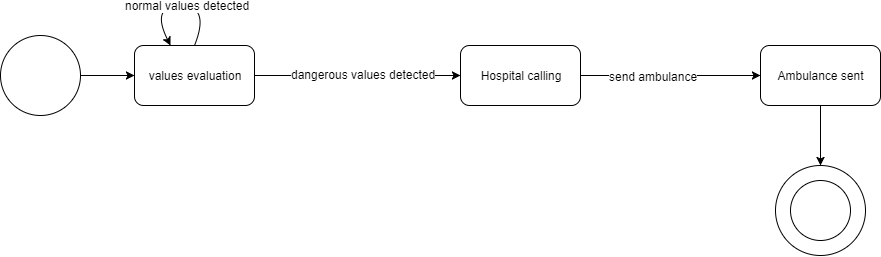
\includegraphics[width=\linewidth]{./Images/Automated_SOS_state_diagram.png}
    \centering
    \caption{AutomatedSOS state diagram}
  \end{figure}


 \begin{figure}[H]
    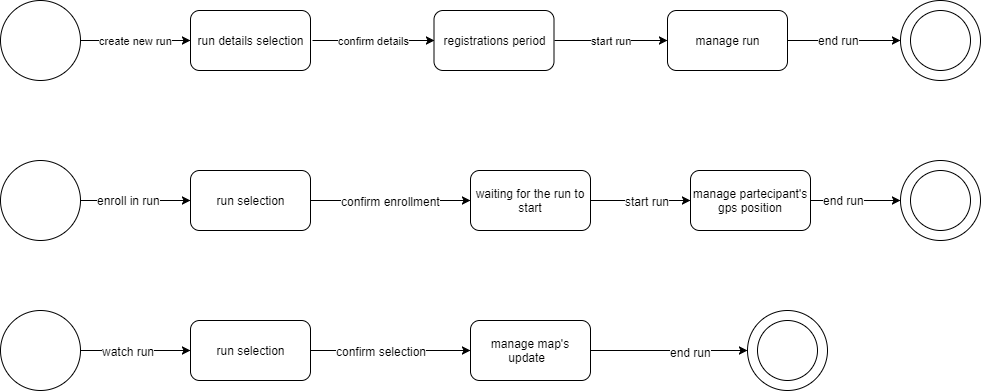
\includegraphics[width=\linewidth]{./Images/Track4Run_state_diagram.png}
    \centering
    \caption{Track4Run state diagram}
  \end{figure}

{\color{secblue}\subsection{Product functions}}
\begin{itemize}
\item The first essential requirement is that all the data must be available remotely for all registered third parties;
\item The second essential requirement is that all the data must be available in a anonymized way, so that no third parties can trace back a specific user data;
\item The third essential requirement is high reliability for the AutomatedSOS service, because of its nature: the service must automatically detect an emergency and act accordingly without the user's interaction. It must be also active 24/7, must have low time response, and must be connected with an automated emergency call service;
\item The fourth essential requirement for the Track4Run service is to be scalable enough for managing any number of active users simultaneously;
\item The fifth essential requirement is that third parties users can have access to all the data from a specific user if that user allow them to do so;
\item The sixth essential requirement is that third parties users can register to a query that was previously requested;
\end{itemize}
{\color{secblue}\subsection{User characteristics}}
Relevant information for each actor:
\begin{itemize}
\item Data4Help Users: these users don't require specific needs, as they only passively contribute to the acquisition of general data for the use of third-parties. Only a smartphone and a smartwatch, or similar device, is required for these users.
\item Registered Third-parties to Data4Help: their need is to be able to acquire various aggregated type of data, filtering their requests based on one or more parameter of the users, like location, personal informations etc. They must receive an answer if the number of results is not too low. Also all answers are anonymized.
\item Users of AutomatedSOS: their need is an application always online which constantly checks their health status and in case of emergency automatically calls an ambulance for them.
\item Users of Track4Run: these users must be able to create a specific track, to browse the available ones, and to join in one or more of them. This user must also be able to be tracked by their position during the run. Also, users that have created a run can join as a partecipant or a spectator as they like.
\end{itemize}
{\color{secblue}\subsection{Assumptions, dependencies and constraints}}
\begin{itemize}
\item D1 - Every user of Data4Help has a smartwatch or a compatible wearable device.
\item D2 - Data acquired through the users' devices is correct and not manipulated.
\item D3 - An automatic ambulance calling service exists. Once the nearest hospital is localized by the system, such service gets called.
\item D4 - The application has access to the ambulance calling system.
\item D5 - The position acquired for tracking each Track4Run's runner is accurate enough, which means that the GPS system needs to be able to track users in a 5 meters diameter.
\end{itemize}
 
%------------------------------------------------------------------------------------------------------------------------------------------------
\clearpage
{\color{secblue}{\section{Specific Requirements}}}
\label{sect:requirements}
\color{black}
{\color{secblue}\subsection{External interface requirements}}
{\color{secblue}\subsubsection{User Interfaces}}

The following mockups offer an intuitive view of what the final product will look like.

\begin{figure}[H]
\centering
\begin{subfigure}{.33\textwidth}
  \centering
  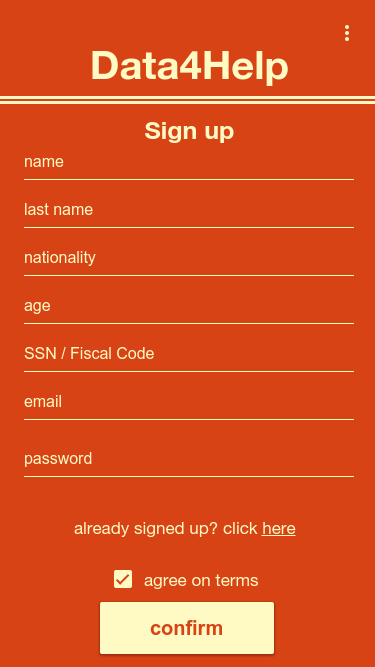
\includegraphics[width=.9\linewidth, height = 7cm, keepaspectratio]{./Images/Mockups/Data4Help/D4HU/D4HU_SignUp.png}
  \caption{Data4Help - User - Sign Up}
\end{subfigure}%
\begin{subfigure}{.33\textwidth}
  \centering
  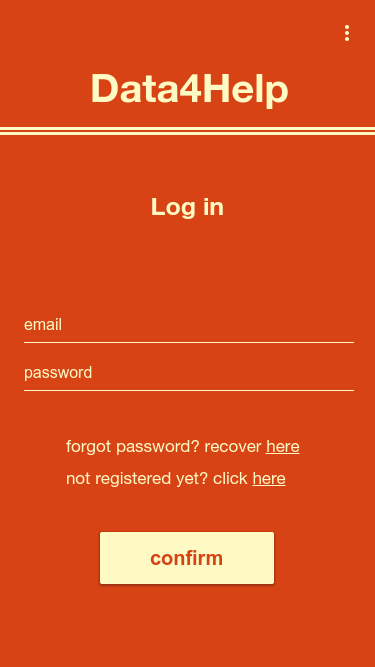
\includegraphics[width = .9\linewidth, height = 7cm, keepaspectratio]{./Images/Mockups/Data4Help/D4HU/D4HU_Login.png}
  \caption{Data4Help - User - Login}
\end{subfigure}
\begin{subfigure}{.33\textwidth}
  \centering
  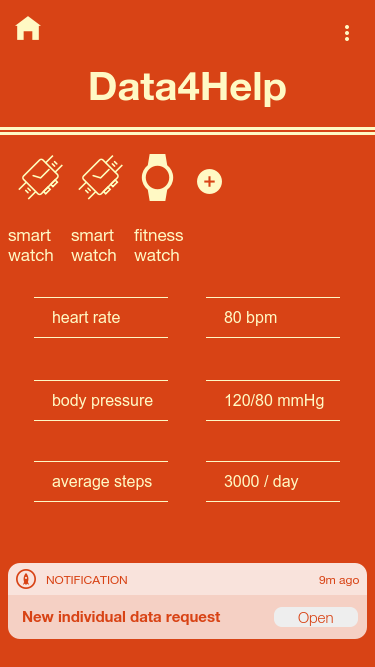
\includegraphics[width = .9\linewidth, height = 7cm, keepaspectratio]{./Images/Mockups/Data4Help/D4HU/D4HU_Homepage.png}
  \caption{Data4Help - User - Homepage}
\end{subfigure}
\end{figure}


\begin{figure}[H]
\centering
\begin{subfigure}{.5\textwidth}
  \centering
  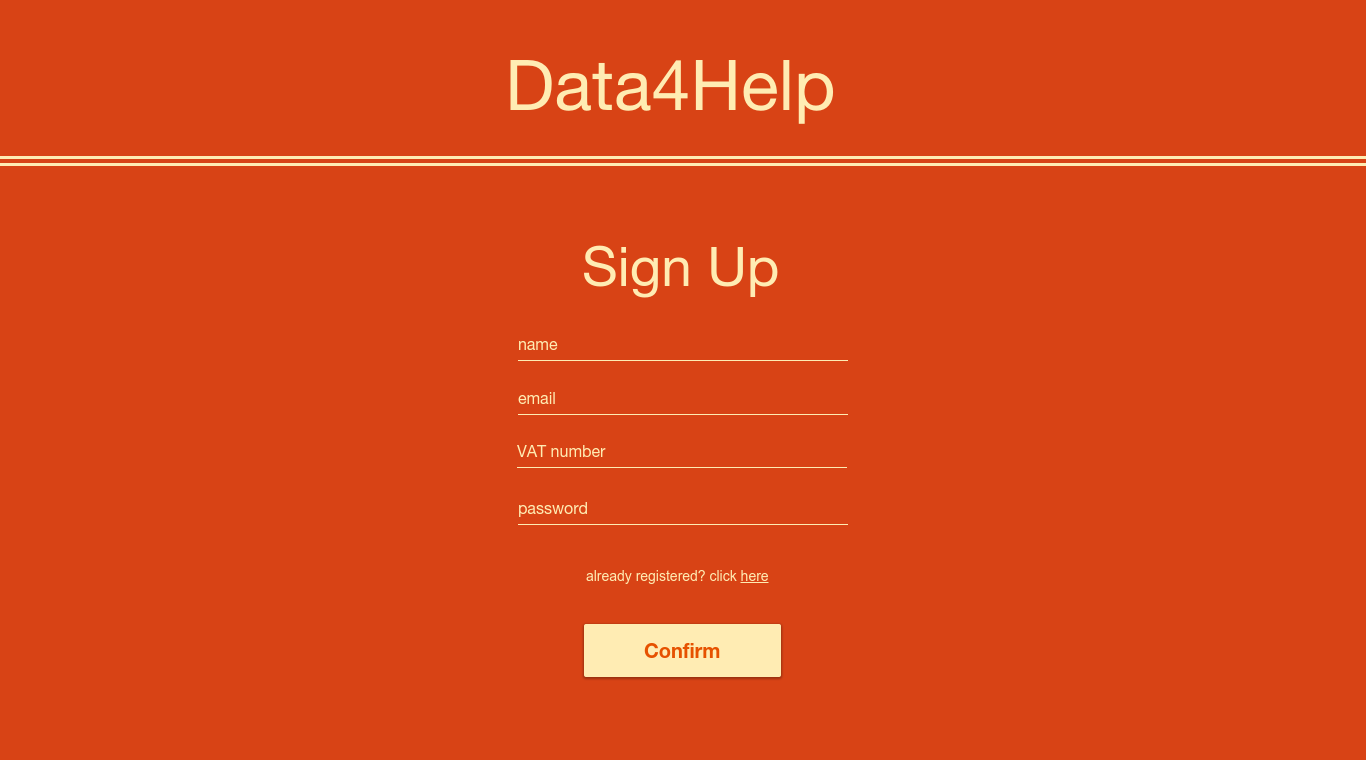
\includegraphics[width=.9\linewidth, height = 7cm, keepaspectratio]{./Images/Mockups/Data4Help/D4HTP/D4HTP_SignUp.png}
  \caption{Data4Help - Third Party - Sign Up}
\end{subfigure}%
\begin{subfigure}{.5\textwidth}
  \centering
  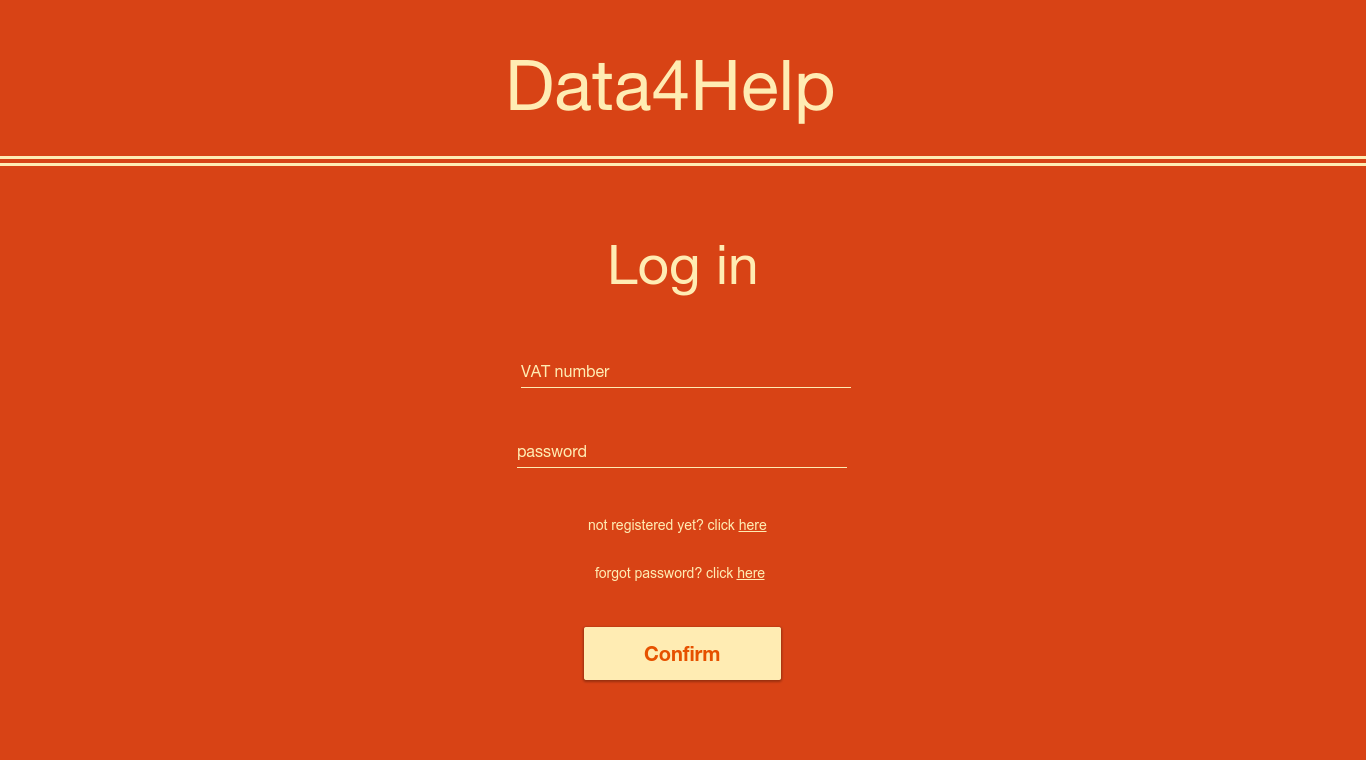
\includegraphics[width = .9\linewidth, height = 7cm, keepaspectratio]{./Images/Mockups/Data4Help/D4HTP/D4HTP_Login.png}
  \caption{Data4Help - Third Party - Login}
\end{subfigure}
\end{figure}

\paragraph{D4HTP - Homepage}
\begin{figure}[H]
    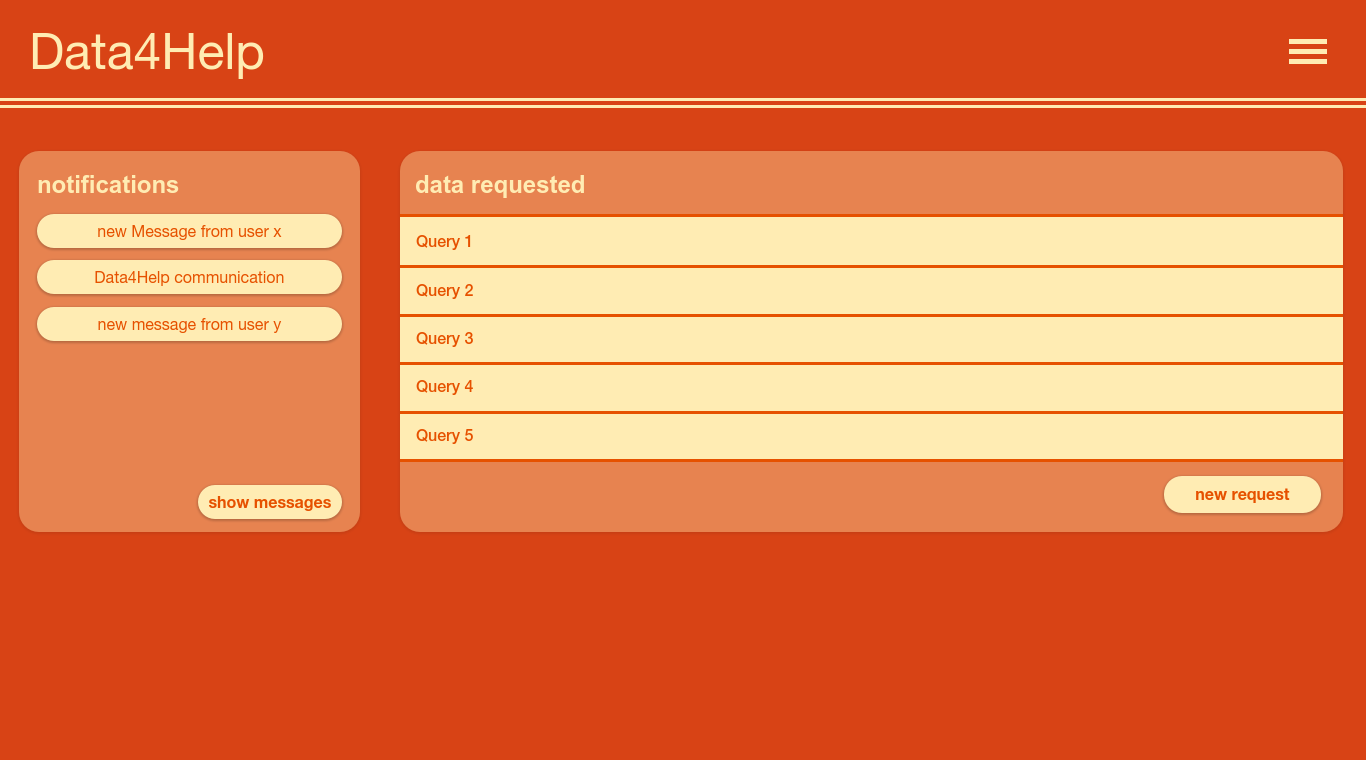
\includegraphics[width=.6\linewidth, height = 20cm, keepaspectratio]{./Images/Mockups/Data4Help/D4HTP/D4HTP_HomePage.png}
    \centering
    \caption{Data4Help - Third Party - Homepage}
    \label{fig:sab}
  \end{figure}

\begin{figure}[H]
    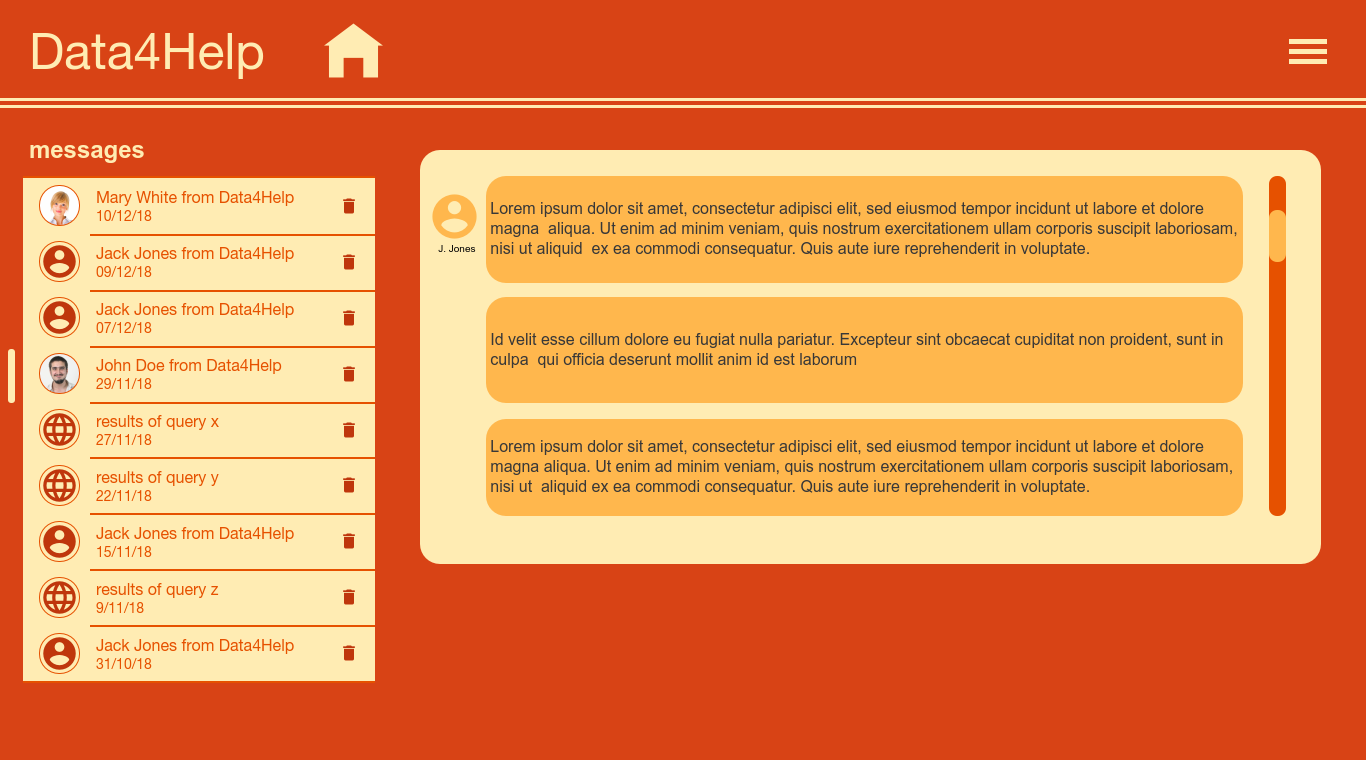
\includegraphics[width=.6\linewidth, height = 20cm, keepaspectratio]{./Images/Mockups/Data4Help/D4HTP/D4HTP_ShowMessages.png}
    \centering
    \caption{Data4Help - Third Party - Messages}
    \label{fig:sab}
\end{figure}


\begin{figure}[H]
    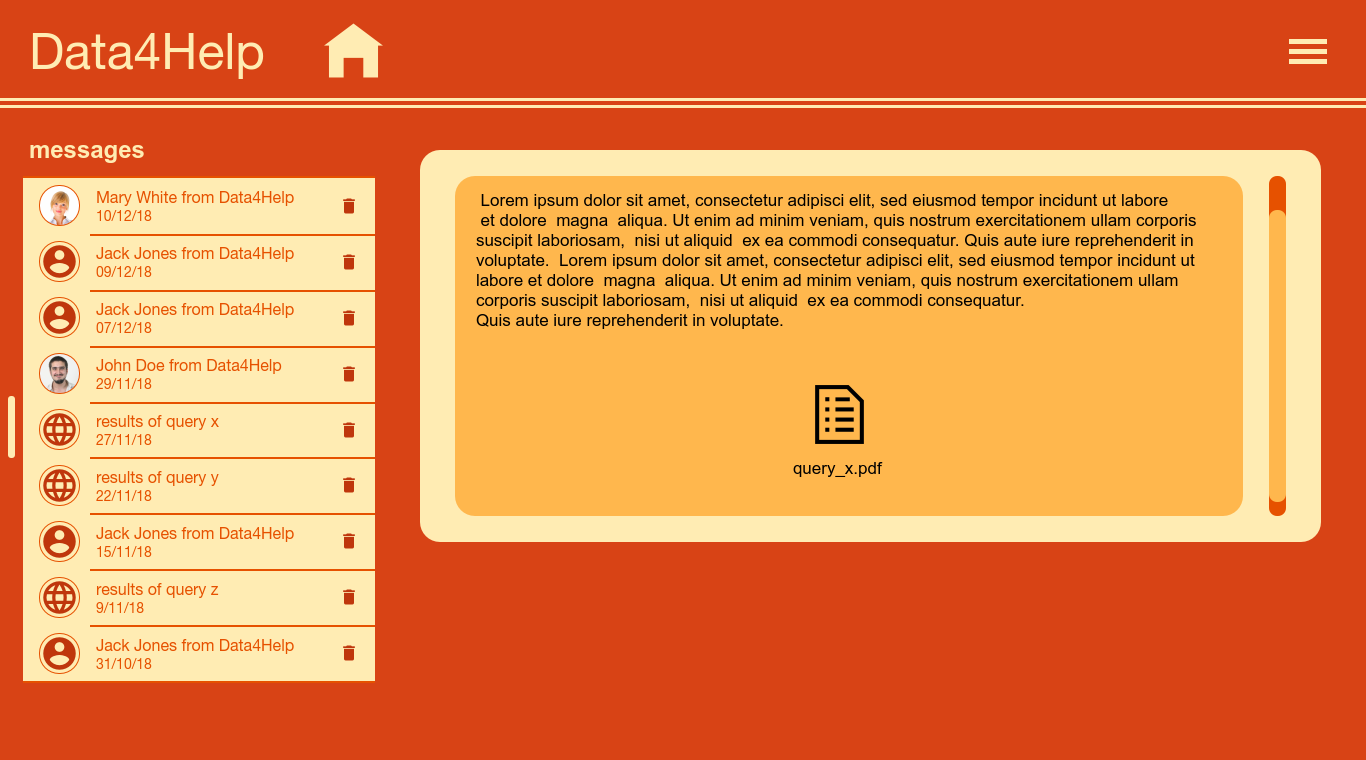
\includegraphics[width=.6\linewidth, height = 20cm, keepaspectratio]{./Images/Mockups/Data4Help/D4HTP/D4HTP_ShowQuery.png}
    \centering
    \caption{Data4Help - Third Party - Messages - Query Result}
    \label{fig:sab}
  \end{figure}


\begin{figure}[H]
    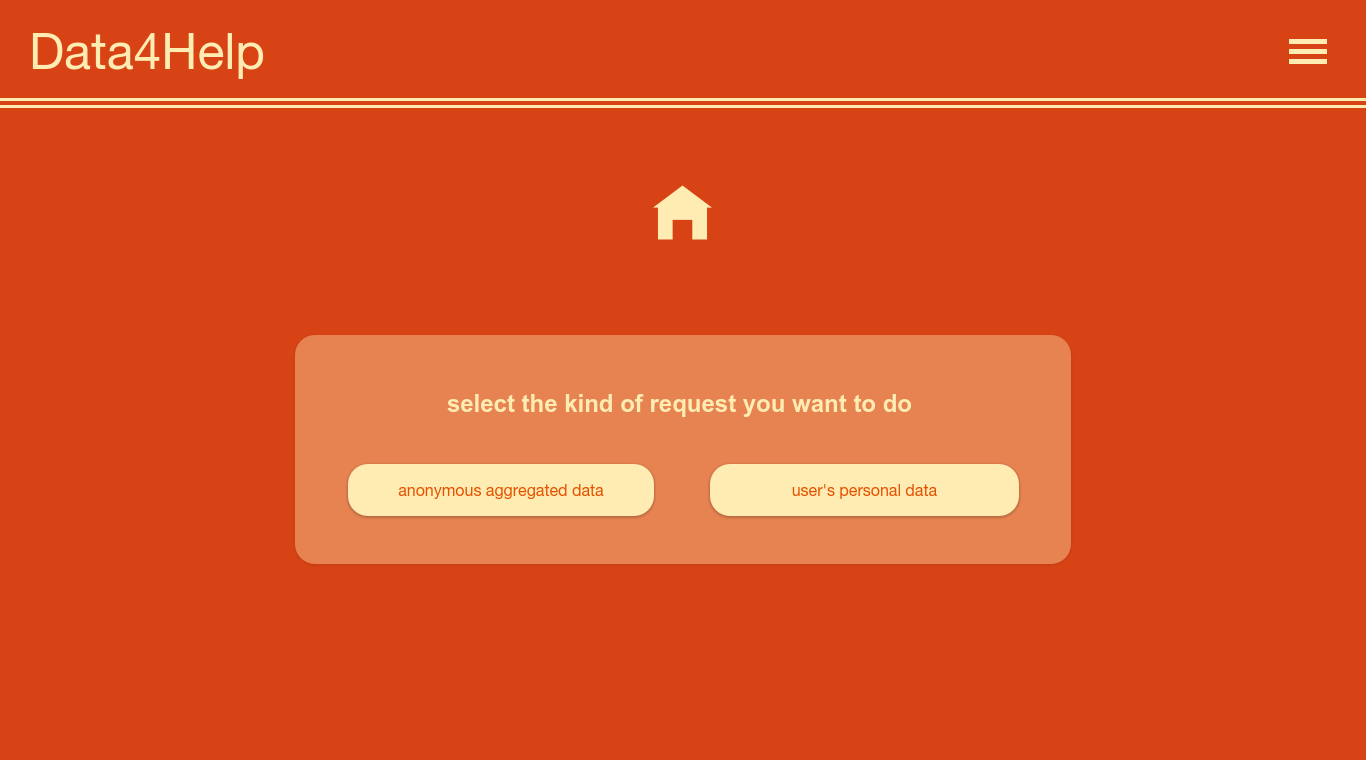
\includegraphics[width=.6\linewidth, height = 20cm, keepaspectratio]{./Images/Mockups/Data4Help/D4HTP/D4HTP_NewQueryRequest.png}
    \centering
    \caption{Data4Help - Third Party - New Query Request}
    \label{fig:sab}
\end{figure}


\begin{figure}[H]
  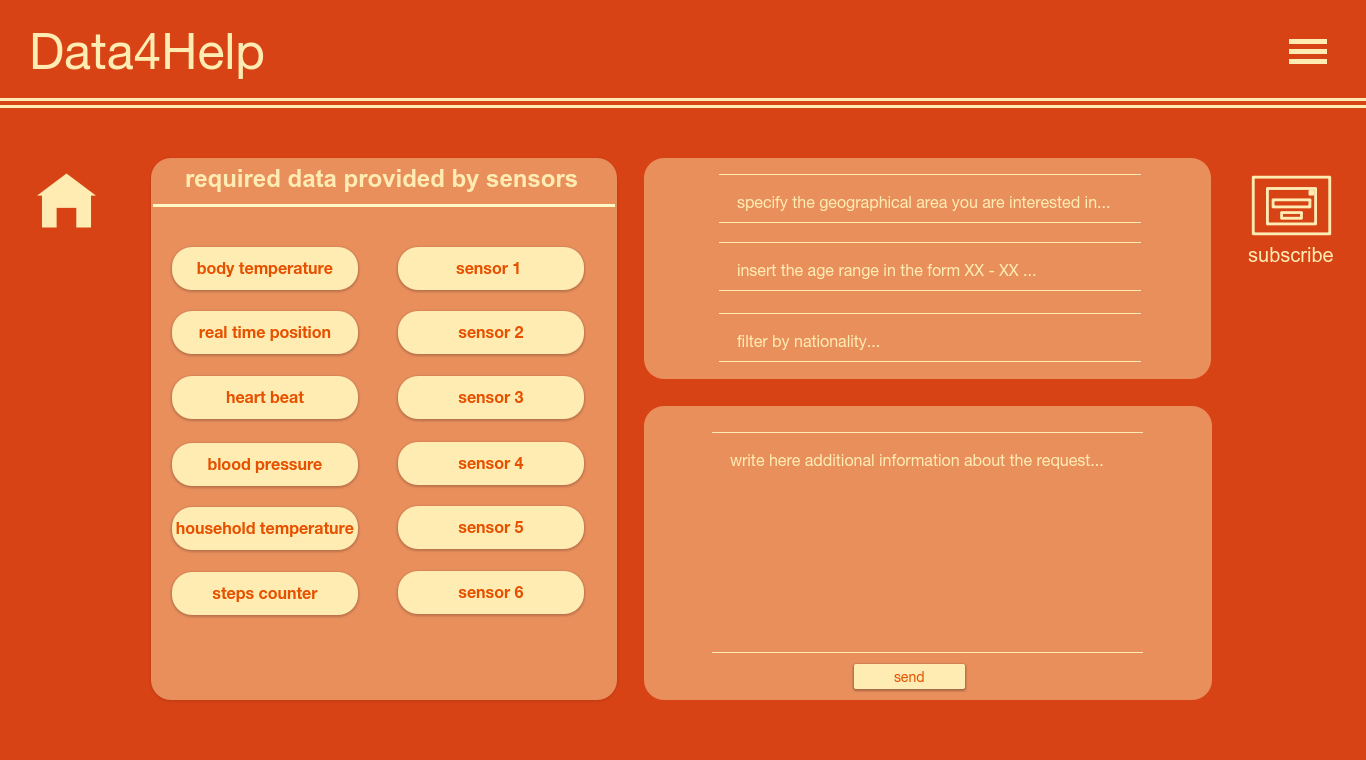
\includegraphics[width=.6\linewidth, height = 20cm, keepaspectratio]{./Images/Mockups/Data4Help/D4HTP/D4HTP_AggregatedDataRequest.png}
  \centering
  \caption{Data4Help - Third Party - Aggregated Data Request}
  \label{fig:sab}
\end{figure}

\begin{figure}[H]
    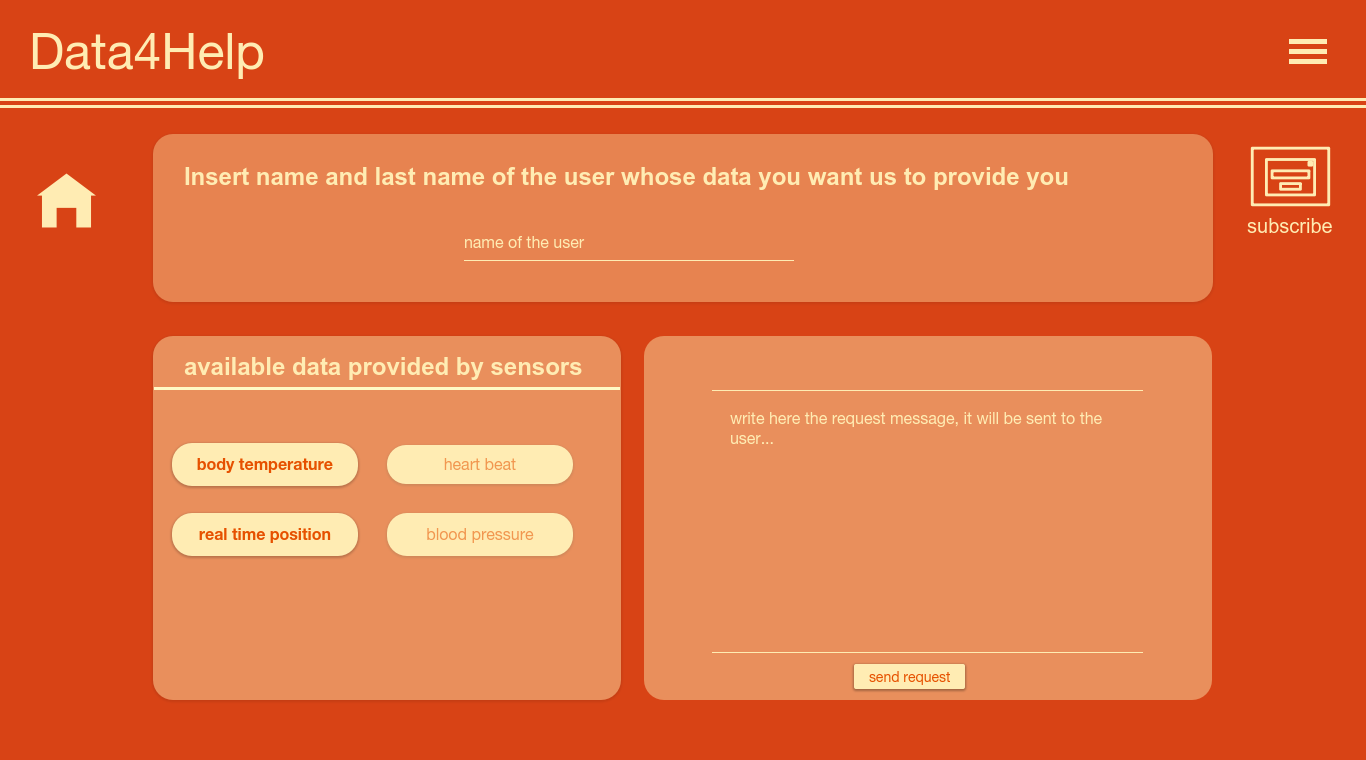
\includegraphics[width=.6\linewidth, height = 20cm, keepaspectratio]{./Images/Mockups/Data4Help/D4HTP/D4HTP_IndividualDataRequest.png}
    \centering
    \caption{Data4Help - Third Party - Individual Data Request}
    \label{fig:sab}
 \end{figure}


\begin{figure}[H]
\centering
\begin{subfigure}{.33\textwidth}
  \centering
  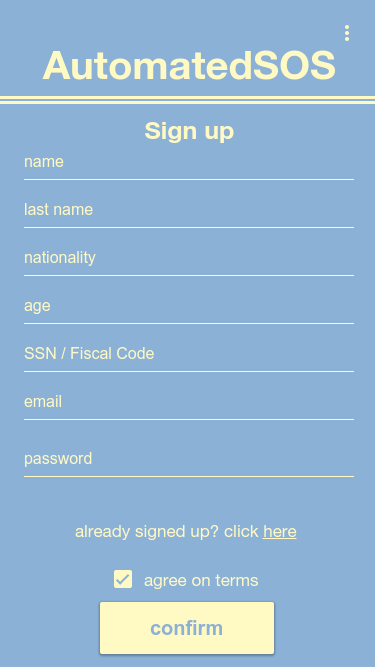
\includegraphics[width=.9\linewidth, height = 7cm, keepaspectratio]{./Images/Mockups/AutomatedSOS/ASOS_SignUp.png}
  \caption{AutomatedSOS - Sign Up}
\end{subfigure}%
\begin{subfigure}{.33\textwidth}
  \centering
  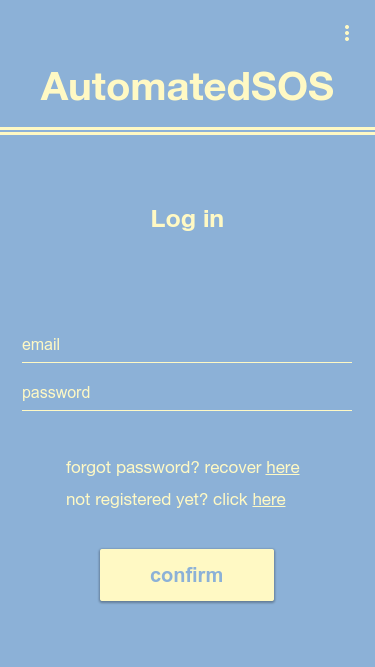
\includegraphics[width = .9\linewidth, height = 7cm, keepaspectratio]{./Images/Mockups/AutomatedSOS/ASOS_Login.png}
  \caption{AutomatedSOS - Login}
\end{subfigure}
\begin{subfigure}{.33\textwidth}
  \centering
  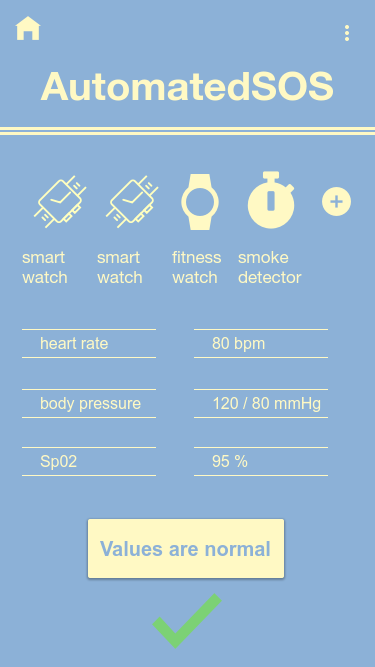
\includegraphics[width = .9\linewidth, height = 7cm, keepaspectratio]{./Images/Mockups/AutomatedSOS/ASOS_Homepage.png}
  \caption{AutomatedSOS - Homepage}
\end{subfigure}
\end{figure}


\begin{figure}[H]
\centering
\begin{subfigure}{.33\textwidth}
  \centering
  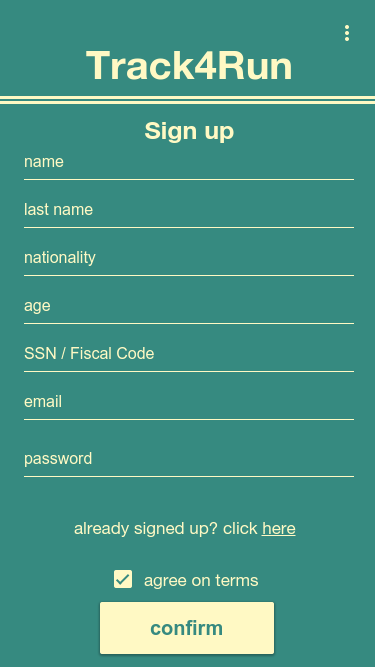
\includegraphics[width=.9\linewidth, height = 6.8cm, keepaspectratio]{./Images/Mockups/Track4Run/T4R_SignUp.png}
  \caption{Track4Run - Sign Up}
\end{subfigure}%
\begin{subfigure}{.33\textwidth}
  \centering
  \includegraphics[width = .9\linewidth, height = 6.8cm, keepaspectratio]{./Images/Mockups/Track4Run/T4R_Login.png}
  \caption{Track4Run - Login}
\end{subfigure}
\begin{subfigure}{.33\textwidth}
  \centering
  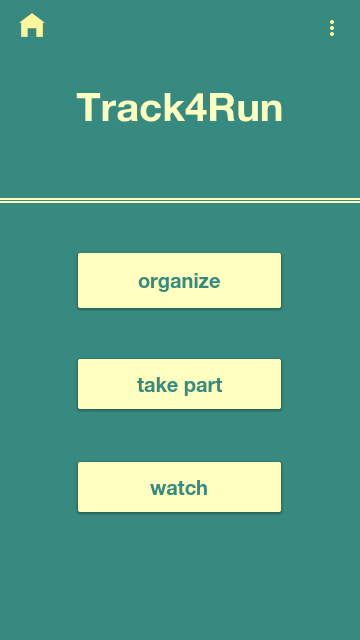
\includegraphics[width = .9\linewidth, height = 6.8cm, keepaspectratio]{./Images/Mockups/Track4Run/T4R_Homepage.png}
  \caption{Track4Run - Homepage}
\end{subfigure}
\end{figure}

\begin{figure}[H]
\centering
\begin{subfigure}{.5\textwidth}
\centering
    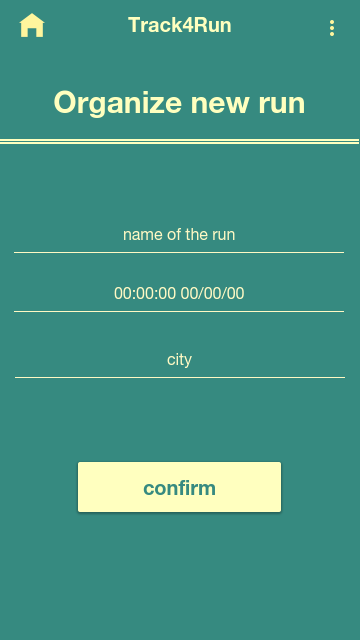
\includegraphics[width=.9\linewidth, height = 6.8cm, keepaspectratio]{./Images/Mockups/Track4Run/T4R_Organize.png}    
    \caption{Track4Run - Organize}
  \end{subfigure}%
\begin{subfigure}{.5\textwidth}
\centering
    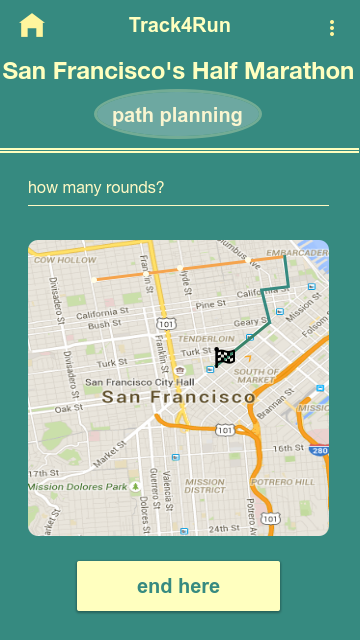
\includegraphics[width=.9\linewidth, height = 6.8cm, keepaspectratio]{./Images/Mockups/Track4Run/T4R_Organize_SetPath.png}
    \caption{Track4Run - Organize - Set Path}
  \end{subfigure}
\end{figure}



\begin{figure}[H]
\centering
\begin{subfigure}{.5\textwidth}
    
\includegraphics[width=.9\linewidth, height = 6.8cm, keepaspectratio]{./Images/Mockups/Track4Run/T4R_TakePart1.png}
    \centering
    \caption{Track4Run - Take Part - Step 1}
  \end{subfigure}%
\begin{subfigure}{.5\textwidth}
    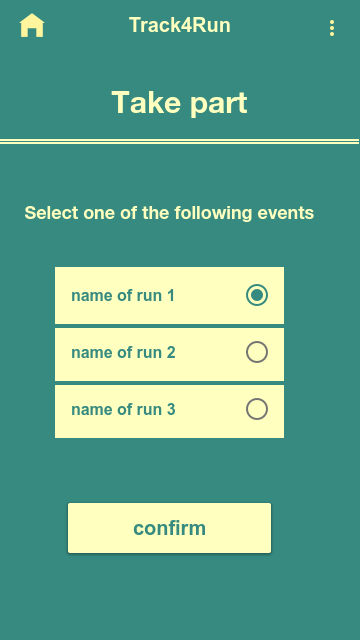
\includegraphics[width=.9\linewidth, height = 6.8cm, keepaspectratio]{./Images/Mockups/Track4Run/T4R_TakePart2.png}
    \centering
    \caption{Track4Run - Take Part - Step 2}
  \end{subfigure}
\end{figure}
  



\begin{figure}[H]
\centering
\begin{subfigure}{.5\textwidth}
    
\includegraphics[width=.9\linewidth, height = 6.8cm, keepaspectratio]{./Images/Mockups/Track4Run/T4R_Watch.png}
    \centering
    \caption{Track4Run - Watch}
  \end{subfigure}%
\begin{subfigure}{.5\textwidth}
    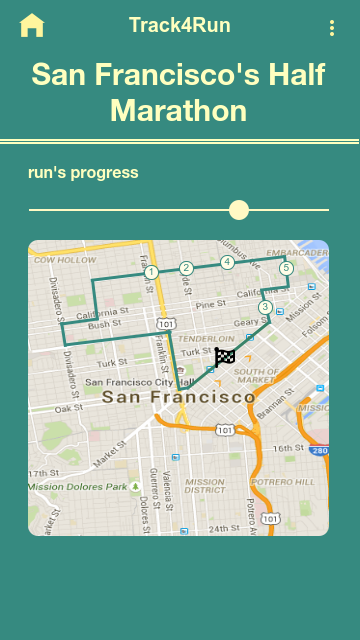
\includegraphics[width=.9\linewidth, height = 6.8cm, keepaspectratio]{./Images/Mockups/Track4Run/T4R_Watch_Map.png}
    \centering
    \caption{Track4Run - Watch - Map}
  \end{subfigure}
\end{figure}


{\color{secblue}\subsubsection{Hardware Interfaces}}
[R1] - This application needs a data warehouse to store all the user data and to allow high performance researchs with large amount of data. This is done using the Amazon AWS services.
{\color{secblue}\subsubsection{Software Interfaces}}
\begin{itemize}
\item{} [R2] - Amazon Redshift as a datawarehouse on top of Amazon S3 to store all the data in an efficent manner;
\item{} [R3] - Google Maps for converting stored GPS data into human readable data for the third parties clients;
\item{} [R4] - Google Maps also for the Track4Run real-time map service.
\item{} [R5] - The API interface for the automatic messagge sent to the nearest hospital.
\end{itemize}
{\color{secblue}\subsubsection{Communication Interfaces}}
[R6] - Both users and third parties will have to use HTTPS to communicate with the TrackMe server, because security and privacy is an important factor in both cases;
\newpage
{\color{secblue}\subsection{Functional requirements}}
{\color{secblue}\subsubsection{Use case diagrams}}
 
\begin{figure}[H]
    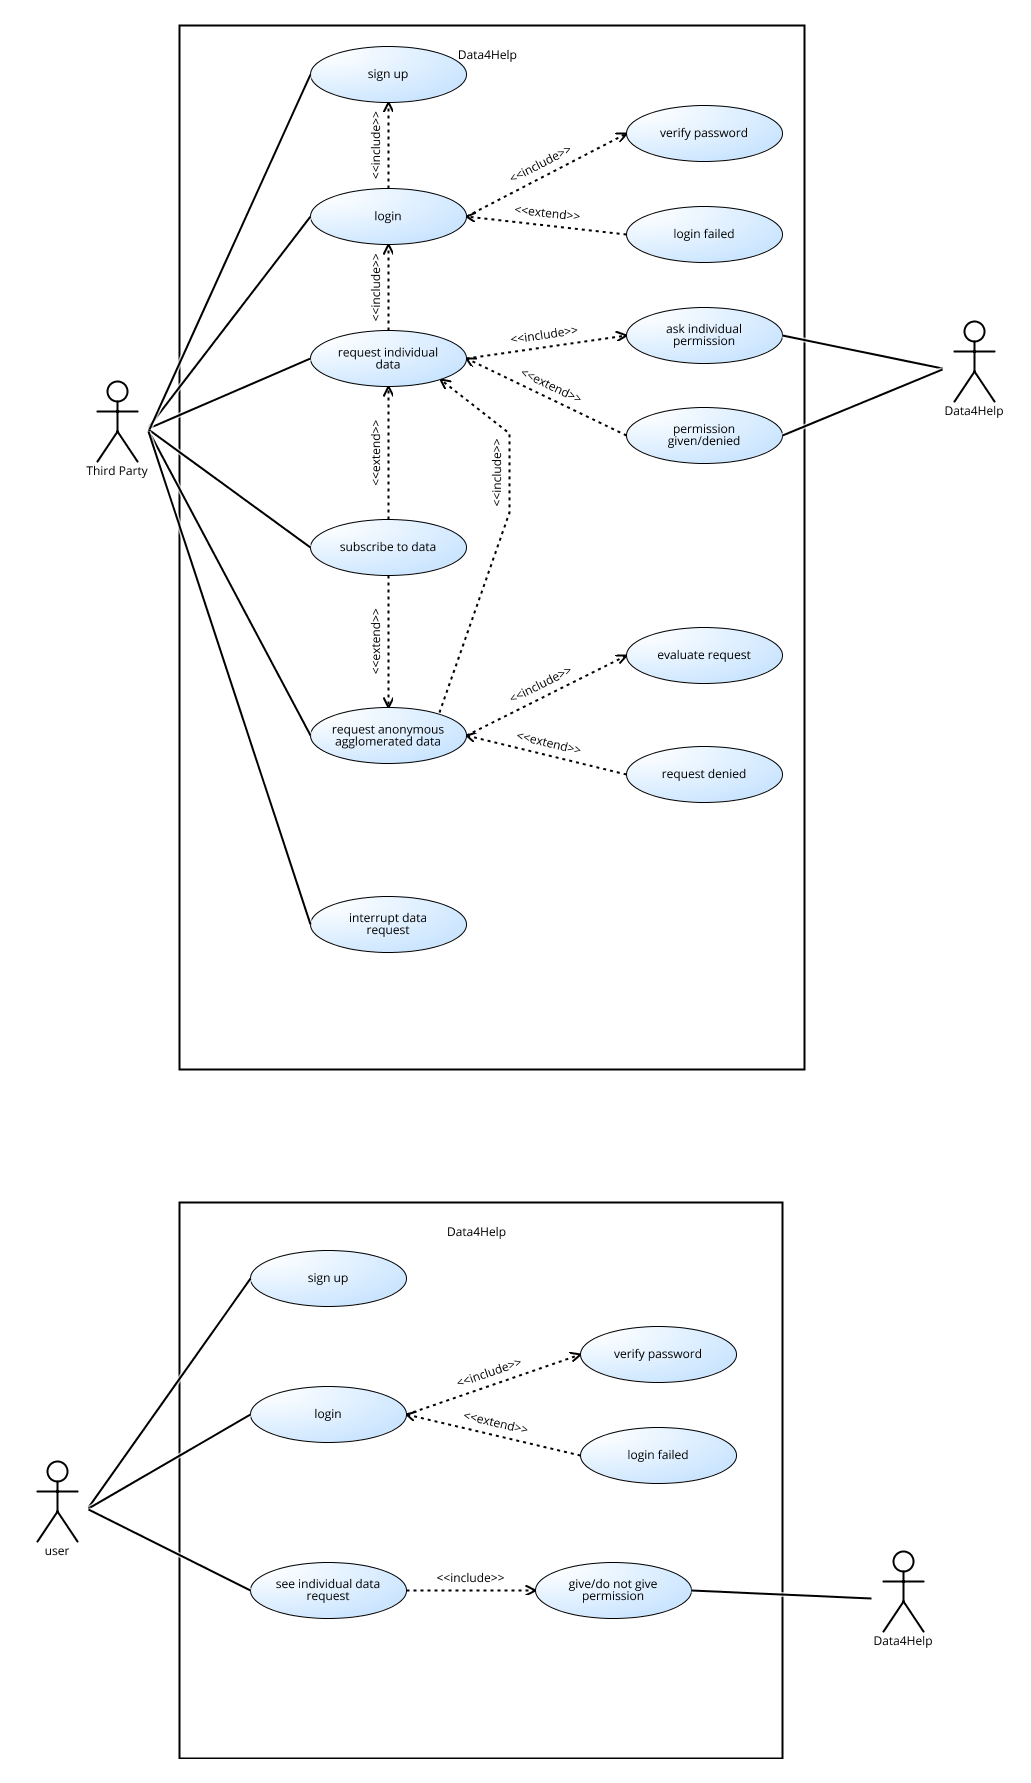
\includegraphics[width=\linewidth, height = 20cm, keepaspectratio]{./Images/RASD_Data4Help_Use_Case_Diagram.png}
    \centering
    \caption{Data4Help}
    \label{fig:sab}
  \end{figure}
\newpage
\begin{figure}[H]
    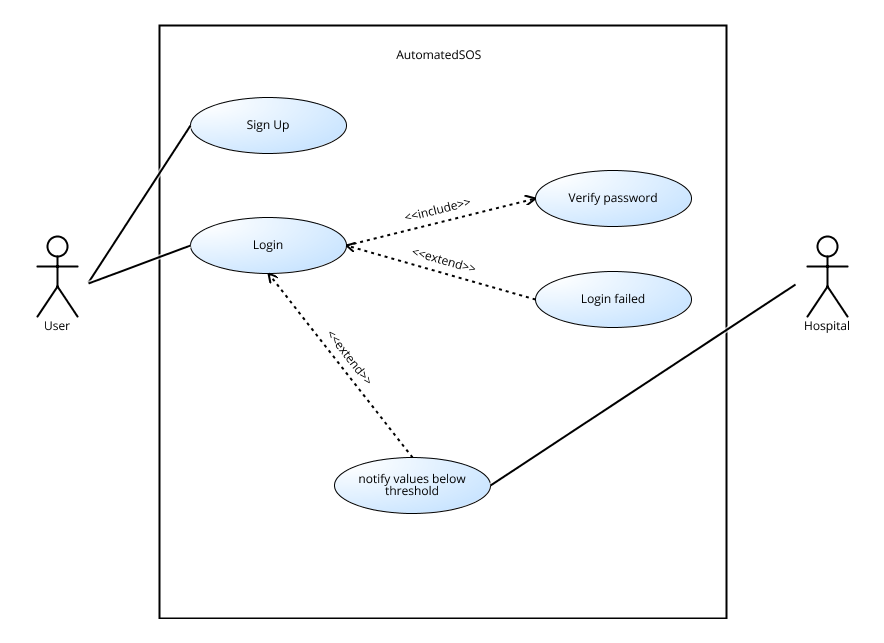
\includegraphics[width=\linewidth, height=10cm, keepaspectratio]{./Images/RASD_Automated_SOS_Use_Case_diagram.png}
    \centering
    \caption{AutomatedSOS}
    \label{fig:sab}
  \end{figure}
  
  
  \begin{figure}[H]
    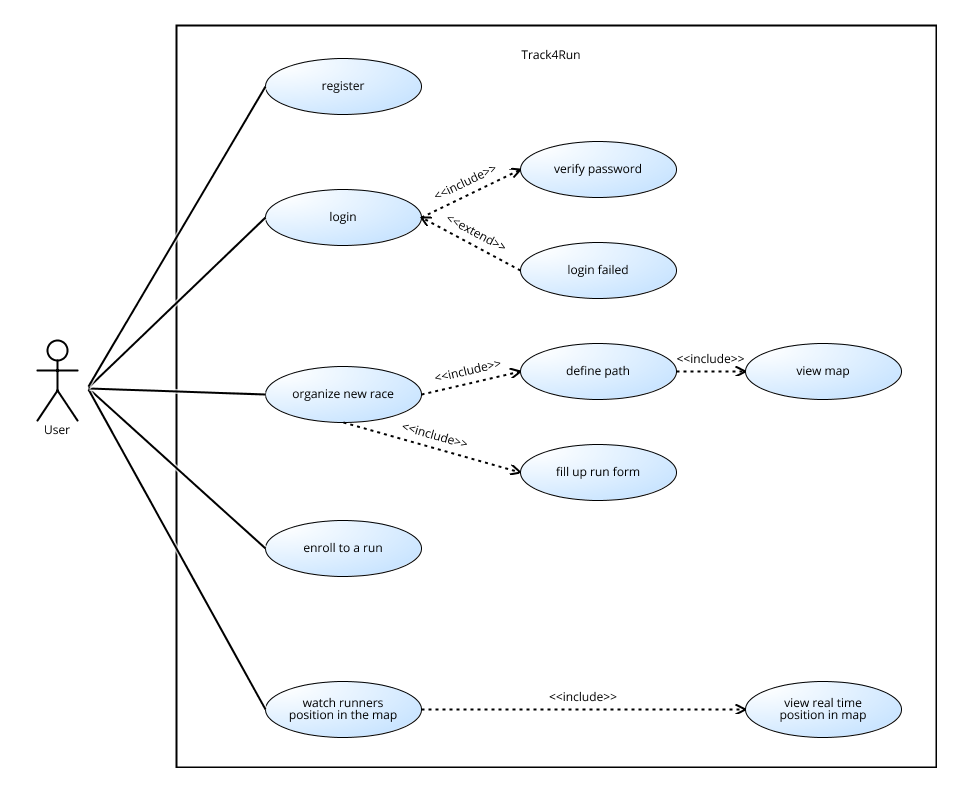
\includegraphics[width=\linewidth, height=10cm, keepaspectratio]{./Images/RASD_Track4Run_Use_Case_Diagram.png}
    \centering
    \caption{Track4Run}
    \label{fig:sab}
  \end{figure}


\begin{table}[]
\begin{tabular}{ll}
\hline
\multicolumn{1}{|l|}{Name}            & \multicolumn{1}{l|}{Sign up - Data4Help}    
 \\ \hline
\multicolumn{1}{|l|}{Actor}           & \multicolumn{1}{l|}{Third Party}                
 \\ \hline
\multicolumn{1}{|l|}{Entry condition} & \multicolumn{1}{l|}{the user has installed the application on his device}                                                                               
 \\ \hline
\multicolumn{1}{|l|}{Event flow}      & \multicolumn{1}{l|}{\begin{tabular}[c]{@{}l@{}}
1. Open the application and click on the "sign in" button\\ 
2. Fill up the form with his personal information, including his fiscal code\\ 
3. Agree with the privacy policy\\ 
4. Confirm the registration\\ 
5. The system saves the data in its database\end{tabular}}                                 
\\ \hline
\multicolumn{1}{|l|}{Exit condition}   & \multicolumn{1}{l|}{The user has successfully registered and is now able to use the service }                                                                                                                      
\\ \hline
\multicolumn{1}{|l|}{Exceptions}       & \multicolumn{1}{l|}{\begin{tabular}[c]{@{}l@{}}All the exceptions are handled by showing to the user a log which\\ explains the kind of exception. Moreover he is taken back to a refreshed\\ "sign up" page.\\ The possible exceptions are:\\ 
1. The email the user provided has already been used\\ 
2. The fiscal code the user provided has already been used \\     
(he has already registered)\\ 
3. The user does not fill all the mandatory info and clicks on "confirm"\\ 
4. The user does not agree with the privacy policy and clicks on "confirm"\end{tabular}}
\\ \hline
\end{tabular}
\end{table}



\begin{table}[]
\begin{tabular}{ll}
\hline
\multicolumn{1}{|l|}{Name}            & \multicolumn{1}{l|}{Login - Data4Help}                        \\ \hline
\multicolumn{1}{|l|}{Actor}           & \multicolumn{1}{l|}{Third Party}                              \\ \hline
\multicolumn{1}{|l|}{Entry condition} & \multicolumn{1}{l|}{the user has installed the application on his PC/Mac, registered and logged in}                                                                                               
\\ \hline
\multicolumn{1}{|l|}{Event flow}      & \multicolumn{1}{l|}{\begin{tabular}[c]{@{}l@{}}
1. Open the application and click on the "login" button\\ 
2. Insert VAT identification number\\ 
3. Insert password\\ 
4. Check VAT and password match\\ 
5. Enter the desktop application\end{tabular}} 
\\ \hline
\multicolumn{1}{|l|}{Exit condition}     & \multicolumn{1}{l|}{The user has successfully logged in and is now on the main page of the application}                                                      
\\ \hline
\multicolumn{1}{|l|}{Exception}          & \multicolumn{1}{l|}{\begin{tabular}[c]{@{}l@{}}All the exceptions are handled by showing to the user a log which\\ explains the kind of exception. Moreover he is taken back to a refreshed\\ "login" page.\\ The possible exceptions are:\\ 
1. The VAT identification number used is unknown by the system\\ 
2. The VAT identification number and the password do not match\\ 
3. The user does not fill the "VAT identification number" field and clicks on "confirm"\\ 
4. The user does not fill the "password" field and clicks on "confirm"\end{tabular}}
\\ \hline
\end{tabular}
\end{table}


\begin{table}[]
\begin{tabular}{ll}
\hline
\multicolumn{1}{|l|}{Name}            & \multicolumn{1}{l|}{Request individual data - Data4Help}     \\ \hline
\multicolumn{1}{|l|}{Actor}           & \multicolumn{1}{l|}{Third Party}                              \\ \hline
\multicolumn{1}{|l|}{Entry condition} & \multicolumn{1}{l|}{the user has installed the application on his PC/Mac, registered and logged in}
\\ \hline
\multicolumn{1}{|l|}{Event flow}      & \multicolumn{1}{l|}{\begin{tabular}[c]{@{}l@{}}
1. Click on the "new request" button from the homepage\\ 
2. Click on the "user's personal data" button \\
2. Fill form with the name of the individual, kind of data requested, \\     and a message to be shown to the individual\\ 
3. Click on the "send request" button\\ 
4. Receive response from the service\end{tabular}}                                      
\\ \hline
\multicolumn{1}{|l|}{Exit condition}     	& \multicolumn{1}{l|}{\begin{tabular}[c]{@{}l@{}}Two possibilities:\\ 
1. The TP receives the approval for the request and the asked data.\\ 
2. The TP receives a denial for the requested data\end{tabular}}                                     \\ \hline
\multicolumn{1}{|l|}{Exceptions}   		& \multicolumn{1}{l|}{\begin{tabular}[c]{@{}l@{}}All the exceptions are handled by showing to the actor a log which\\ explains the kind of exception. Moreover he is taken back to a refreshed\\ "request individual data" page.\\ The possible exceptions are:\\ 
1. The name inserted in the form does not match with any \\ name contained in the database\end{tabular}}
\\ \hline
\end{tabular}
\end{table}




\begin{table}[]
\begin{tabular}{ll}
\hline
\multicolumn{1}{|l|}{Name}            & \multicolumn{1}{l|}{Request anonymous aggregated data - Data4Help}                                                                                            \\ \hline
\multicolumn{1}{|l|}{Actor}           & \multicolumn{1}{l|}{Third Party}                              \\ \hline
\multicolumn{1}{|l|}{Entry condition} & \multicolumn{1}{l|}{the third party has installed the application on his PC/Mac, registered and logged in} 
\\ \hline
\multicolumn{1}{|l|}{Event flow}      & \multicolumn{1}{l|}{\begin{tabular}[c]{@{}l@{}}
1. Click on the "new request" button from the homepage\\ 
2. Click on the "anonymous aggregated data" button\\
3. Specify the kind of data requested (position, age, average heart beat rate,...)\\ 
4. Click on the "send" button\\ 
5. Receive response from the service\end{tabular}}  
\\ \hline
\multicolumn{1}{|l|}{Exit condition}    & \multicolumn{1}{l|}{\begin{tabular}[c]{@{}l@{}}Two possibilities:\\ 
1. The third party receives the approval for the request and the asked data.\\ 
2. The third party receives a denial for the requested data, because\\     the number of individual registered in such area that satisfies the criteria\\     chosen by the third party are less the 1000\end{tabular}}
\\ \hline
\multicolumn{1}{|l|}{Exceptions}         & \multicolumn{1}{l|}{\begin{tabular}[c]{@{}l@{}}All the exceptions are handled by showing to the user a log which\\ explains the kind of exception. Moreover he is taken back to a refreshed\\ "aggregated data request" page.\\ The possible exceptions are:\\ 
1. No data is requested from the third party and the "send" button is clicked\end{tabular}}
\\ \hline
\end{tabular}
\end{table}


\begin{table}[]
\begin{tabular}{ll}
\hline
\multicolumn{1}{|l|}{Name}            & \multicolumn{1}{l|}{Sign up - AutomatedSOS \& Track4Run}     \\ \hline
\multicolumn{1}{|l|}{Actor}           & \multicolumn{1}{l|}{User}                                     \\ \hline
\multicolumn{1}{|l|}{Entry condition} & \multicolumn{1}{l|}{the user has installed the app on his device}                                                                                               \\ \hline
\multicolumn{1}{|l|}{Event flow}      & \multicolumn{1}{l|}{\begin{tabular}[c]{@{}l@{}}
1. Click on the "sign up" button \\ 
2. Fill up the form with personal info \\ 
3. Click on the "confirm" button\end{tabular}}                                                        \\ \hline
\multicolumn{1}{|l|}{Exit condition}      & \multicolumn{1}{l|}{The user signs up and is ready to log in}
\\ \hline
\multicolumn{1}{|l|}{Exceptions}           & \multicolumn{1}{l|}{ \begin{tabular}[c]{@{}l@{}}All the exceptions are handled by showing to the user a log which\\ explains the kind of exception. Moreover he is taken back to a refreshed\\ "sign up" page.\\ The possible exceptions are:\\ 
1. The user does not fill all the mandatory information in the form and\\     clicks on the "confirm" button\\ 
2. The user does not agree with the privacy policy and clicks on the \\     confirm button\end{tabular}}
\\ \hline
\end{tabular}
\end{table}



\begin{table}[]
\begin{tabular}{ll}
\hline
\multicolumn{1}{|l|}{Name}            & \multicolumn{1}{l|}{Login - AutomatedSOS \& Track4RUn}        \\ \hline
\multicolumn{1}{|l|}{Actor}           & \multicolumn{1}{l|}{User}                                     \\ \hline
\multicolumn{1}{|l|}{Entry condition} & \multicolumn{1}{l|}{the user has installed the app on his device and signed up}                                                                                 \\ \hline
\multicolumn{1}{|l|}{Event flow}      & \multicolumn{1}{l|}{\begin{tabular}[c]{@{}l@{}}
1. Click on the "login" button \\ 
2. Insert email\\ 
3. Insert password\\ 
4. Click on the "confirm" button\end{tabular}}                                                        \\ \hline
\multicolumn{1}{|l|}{Exit condition}    & \multicolumn{1}{l|}{The user logs in  and is ready to use the service}
\\ \hline
\multicolumn{1}{|l|}{Exceptions}         & \multicolumn{1}{l|}{\begin{tabular}[c]{@{}l@{}}All the exceptions are handled by showing to the user a log which\\ explains the kind of exception. Moreover he is taken back to a refreshed\\ "login" page.\\ The possible exceptions are:\\ 
1. The user inserts an e-mail address unknown by the system's database\\ 
2. The user inserts a known e-mail address but the password he inserts \\     does not match the provided e-mail\end{tabular}}
\\ \hline
\end{tabular}
\end{table}


\begin{table}[]
\begin{tabular}{ll}
\hline
\multicolumn{1}{|l|}{Name}            & \multicolumn{1}{l|}{Organize new run - Track4Run}             \\ \hline
\multicolumn{1}{|l|}{Actor}           & \multicolumn{1}{l|}{User}                                     \\ \hline
\multicolumn{1}{|l|}{Entry condition} & \multicolumn{1}{l|}{the user has installed and logged in the application on his device}                                                                            \\ \hline
\multicolumn{1}{|l|}{Event flow}      & \multicolumn{1}{l|}{\begin{tabular}[c]{@{}l@{}}1. Click on the "organize" button\\ 2. Fill up form with name of the event, date, location\\ 3. Click on the "confirm" button\\ 4. Select path from available paths by:\\ 4a. choosing start point from available street\\ 4b. choosing end point from such street\\ 5. Choose between going back to 4a. or ending path\\ 6. Click on the "confirm" button\end{tabular}}                                                     \\ \hline
\multicolumn{1}{|l|}{Exit condition}     & \multicolumn{1}{l|}{The user has successfully organized the run}
\\ \hline
\multicolumn{1}{|l|}{Exception}       & \multicolumn{1}{l|}{\begin{tabular}[c]{@{}l@{}}All the exceptions are handled by showing to the user a log\\ which explains the kind of exception. Moreover he is taken back\\ to a new "Organize new run" page.\\ The possible exceptions are:\\ 1. The user forgets to fill at least one of the field in the form and\\     clicks on the "confirm" button.\\ 2. The city selected to organize the run in is not recognized\\      by the Track4Run systems, which means that Track4Run\\     does not own a stylized map of such city.\end{tabular}}
\\ \hline
\end{tabular}
\end{table}

\newpage

{\color{secblue}\subsubsection{Sequence diagrams}}

\begin{figure}[H]
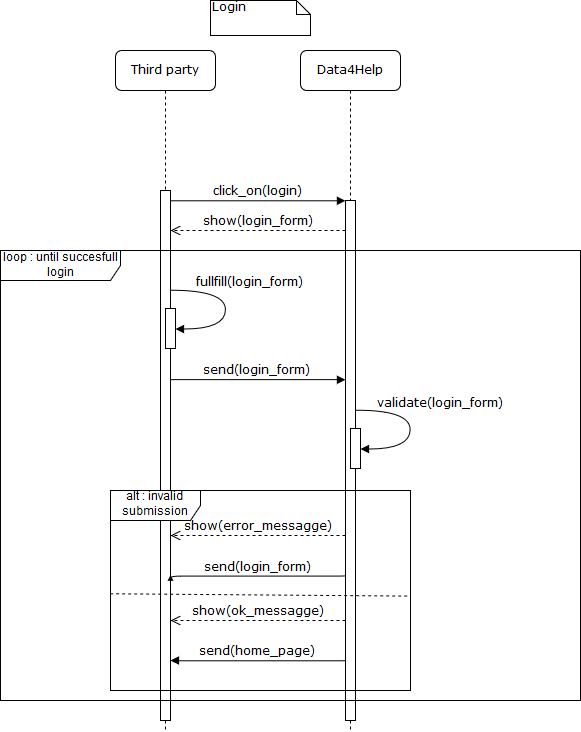
\includegraphics[width=\linewidth, height=9cm, keepaspectratio]{./Images/sequence_diag_login.png}
\centering
\caption{Login sequence diagram}
\end{figure}

\begin{figure}[H]
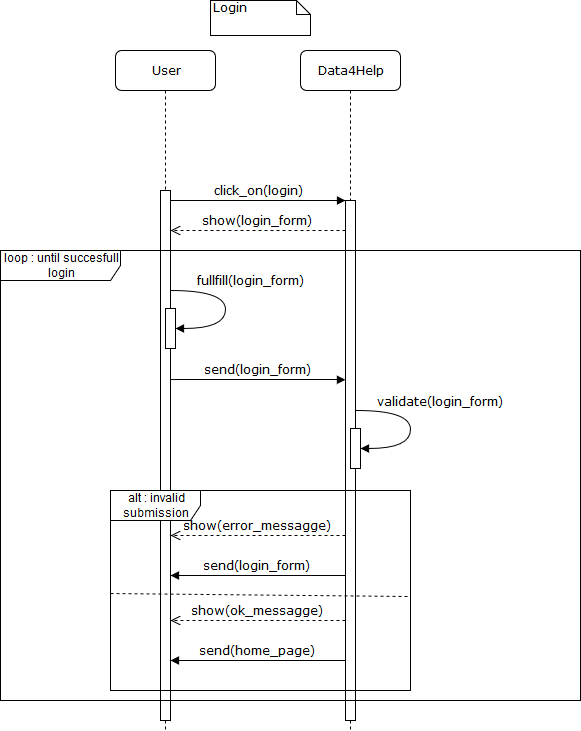
\includegraphics[width=\linewidth, height=9cm, keepaspectratio]{./Images/sequence_diag_login_user.png}
\centering
\caption{User's login sequence diagram}
\end{figure}

\begin{figure}[H]
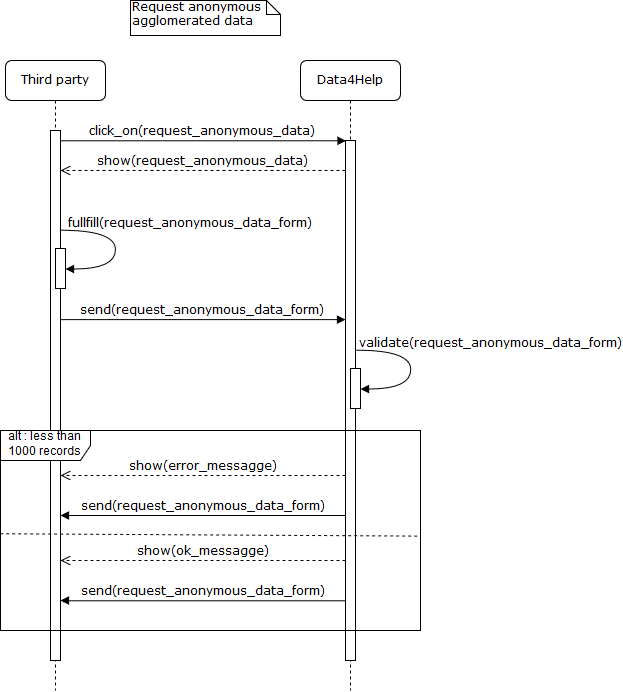
\includegraphics[width=\linewidth, height=9cm, keepaspectratio]{./Images/sequence_diag_request_anonymous_agglomerated_data.png}
\centering
\caption{Request anonymous agglomerated data sequence diagram}
\end{figure}

\begin{figure}[H]
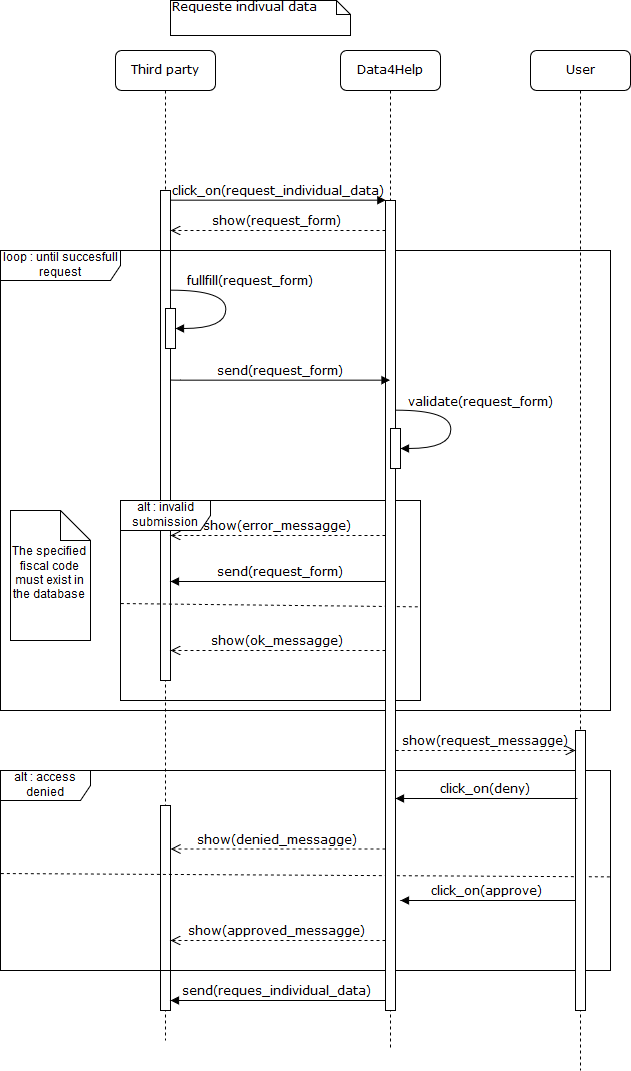
\includegraphics[width=\linewidth, height=11cm, keepaspectratio]{./Images/sequence_diag_request_individual_data.png}
\centering
\caption{Request individual data sequence diagram}
\end{figure}

\begin{figure}[H]
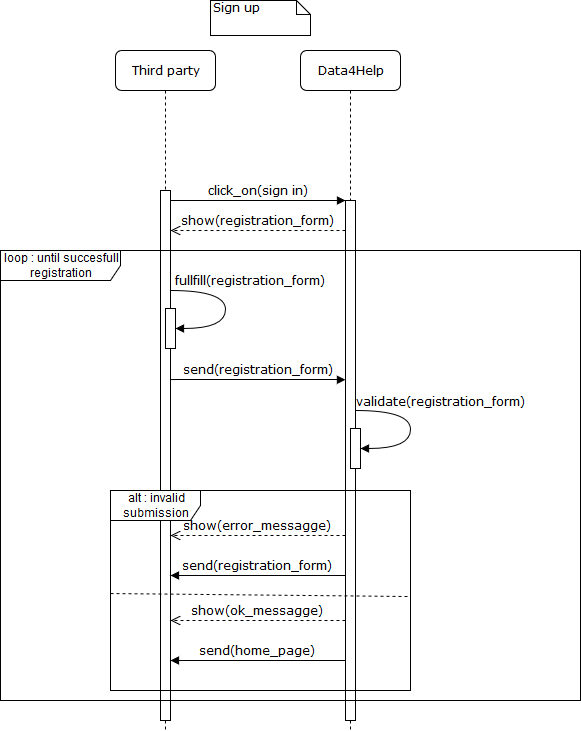
\includegraphics[width=\linewidth, height=10cm, keepaspectratio]{./Images/sequence_diag_sign_up.png}
\centering
\caption{Sign up sequence diagram}
\end{figure}

\begin{figure}[H]
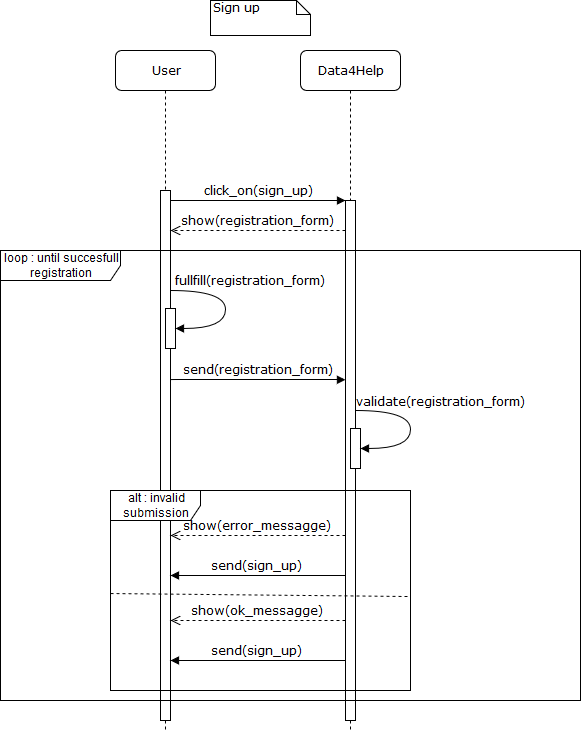
\includegraphics[width=\linewidth, height=10cm, keepaspectratio]{./Images/sequence_diag_sign_up_user.png}
\centering
\caption{Sign up user sequence diagram}
\end{figure}

\begin{figure}[H]
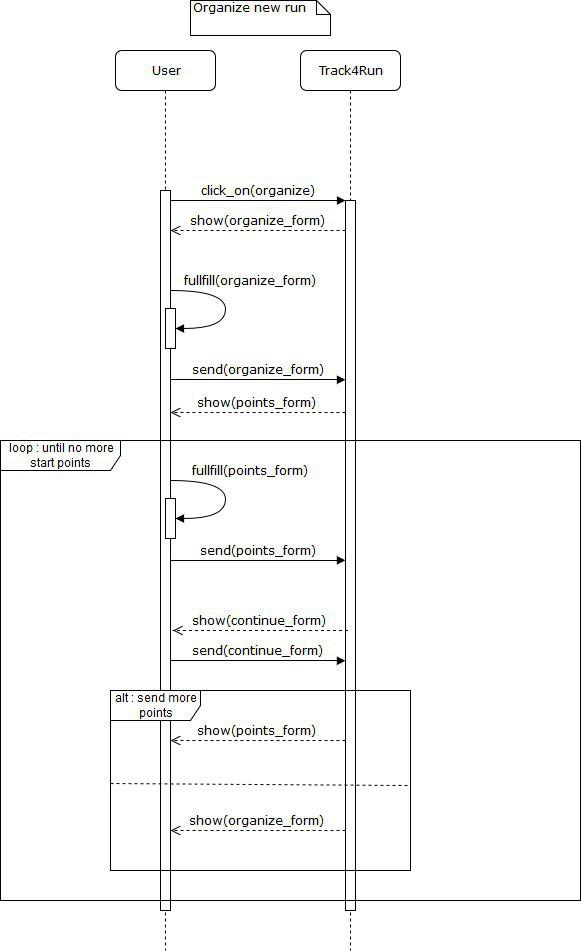
\includegraphics[width=\linewidth, height=10cm, keepaspectratio]{./Images/sequence_diag_new_run.jpg}
\centering
\caption{New run sequence diagram}
\end{figure}
\newpage
{\color{secblue}\subsubsection{Mapping on requirements}}
\begin{itemize}
\item [G1] - The Data4Help application gives constantly new data accordingly to users' activities.
This is achieved with [D1], [D2], [R8], [R9], [R10], [R11], [R13], [R14],\\
\textbf{[FR1]} - The users must be logged in
\item [G2] - Registered TPs (Third Parties) can send request to specific users if they know their SSN or CF to retrieve their specific data.
This is achieved with [R2], [R3], [R8], [R10], [FR1], \\
\textbf{[FR2]} - the users have the possibility of accepting or refusing a non-anonymous data requests. \newline
\textbf{[FR3]} - The TP must be logged in.


\item [G3] - Registered TPs have access to make queries to Data4Help's database to get specific data by filtering by one or more parameters as they need.
This is achieved with [D2], [R1], [R2], [R3], [R7], [R8], [R10], [R11], [FR3]


\item [G4] - Results for TPs' queries are given only if the number of matches is greater or equal than 1000.
This is achieved with [R1], [R2], [R7].


\item [G5] - Each user of the services offered by TrackMe is identifiable in order to gather his data and to communicate with him.
This is achieved with 
[R6], [FR1], [R12], \\
\textbf{[FR4]} - the users must register in the system in order to be identified.

\item [G6] AutomatedSOS sends automatically a request when and only when some user's values are below a specific critical threshold, specifying the user's position.
This is achieved with [D1], [D2], [D3], [D4], [R5], [R6], [R9], [R10], [R11], [R14], [FR1], \\
\textbf{[FR5]} - The hospitals need to be always available in case of emergency call, this means that there is always an ambulance and some personnel available. \\
\textbf{[FR6]} - The users of AutomatedSOS need to have their sensors equipped devices connected to the system in order to be helped.


\item [G7] - Users of Track4Run are able to create a run defining the precise path.
This is achieved with [R1], [R6], [R7], [R14], [FR1], \\
\textbf{[FR7]} - The users of Track4Run, whenever they want to organize a new run, need to insert reasonable gps coordinates in the definition of the path. \\
\textbf{[FR8]} - The users of Track4Run, whenever they want to organize a new run, need to have the permission of the city hall in case the path defined is public land.
\item [G8] - Users of Track4Run are able to take part in a created run as runners.
This is achieved with [R7], [R14], [FR1], \\
\textbf{[FR9]} - The users of Track4Run, whenever they take part in a run, need to wear their gps equipped device in order to be tracked.
\item [G9] - Users of Track4Run can see real-time runners' positions of runs in which they are subscribed.
This is achieved with [D5], [R4], [R7], [R11].
\end{itemize}

{\color{secblue}\subsection{Performance requirements}}
[R7] - Performance plays a big role in all the 3 projects: regarding the Data4Help and Track4Run they both have to manage a large amount of people that can range from 0 (i.e.: an event organized through Track4Run) to 10000 (i.e.: a fair amount of user that we should excpect from Data4Help) based on the current users requests. Regarding the AutomatedSOS there isn't a specific need for performance, but for reliability, which is explained in the reliability section.
{\color{secblue}\subsection{Design constraints}}
{\color{secblue}\subsubsection{Standard compliance}}
[R8] - Internally the data that is collected through Data4Help can be stored in any way that is comfortable for the developers to work with, but when it is delivered to the third parties it must use a standard format.
This means that:
\begin{enumerate}
\item - R8.1 - the TP can choose of receiving the results of its requests in the form of a summary in a PDF file.
\item - R8.2 - the TP can choose of receiving the results of its request in a database file, in such a way that the third parties can manipulate the data the way they like.
\item - R8.3 - The TP can request both the formats above.
\end{enumerate}
{\color{secblue}\subsubsection{Hardware limitations}}
The services to be developed would work on any of the smartphones available in the market because the technologies needed for such services in order to work are very basic (bluetooth connection with the sensors equipped devices, gps and internet connection).

{\color{secblue}\subsubsection{Any other constraints}}
[R9] - Bandwidth may be a constraint, because developers need to pay attention to send only the essential data from the sensors equipped device to the server, because in an hypotetical situation the application may drain too much mobile data from the users' sensors equipped device. To achieve this is possible also to set a reasonable amount of time to be waited between each single user's update of his/her values to the server. On the contrary, AutomatedSOS doesn't have any bandwidth limitation.
{\color{secblue}\subsection{Software system attributes}}
{\color{secblue}\subsubsection{Reliability}}
[R10] - Reliability is the main concern for AutomatedSOS, because of the nature of the service itself, and surely is important in the development of the Data4Help module. Secondly, reliability is not the main concern in Track4Run.
The whole system should at least be 99.999\% reliable.
{\color{secblue}\subsubsection{Availability}}
[R11] - AutomatedSOS needs a six 9s (99.9999\%) availability, due to the high importance availability plays for this service, while Data4Help and AutomatedSOS need at least a five 9s (99.999\%) availability.
{\color{secblue}\subsubsection{Security}}
[R12] - Anonymization must be granted giving the fact that we are working with very sensible data.
Since AutomatedSOS and Track4Run talk with Data4Help, this means that the communication between the modules must be protected as well. 

{\color{secblue}\subsubsection{Mantainability}}
[R13] - Mantainability is a big concern for all the three services. Given the fact that the application is mainly developed for Android and iOS, it must be easily maintainable, because of the frequent updates of both the operating systems. This translates in the decoupling of the components of the system.

{\color{secblue}\subsubsection{Portability}}
[R14] - The application that is developed for Data4Help users must work for all iOS' and Android's updates by the date of launch of the app. The same can be applied to Track4Run and Automated SOS because it's not easy to foresee how smartwatches' and smartphones' market will change in the future. The desktop application of Data4Help instead has not the same portability requirements, because, being developed for the Windows operating system, we can rely on his well established legacy of portability.
{\color{secblue}\subsection{Scenarios}}
{\color{secblue}\subsubsection{Scenario 1 - Data4Help}}
Data Request:
A local newspaper of the city of Padova wants to write an article about the average 
age of the people visiting the city so one of the journalists opens the Data4Help account of his journal on his PC.
He finds himself in the homepage of the application and clicks on the "New Request" button. Then He clicks on the "anonymous aggregated data" button.
Afterwards a few text fields pop up and he fills them with requesting to the system the age of the people that in the last month
spent at most one week in the city. Done so, he asks for a monthly update. He clicks on "send" and waits for the approval of the request.
After a few seconds the system approves the request and provides him with a list of numbers corresponding to the ages of such people (such list is provided monthly as requested).


{\color{secblue}\subsubsection{Scenario 2 - Data4Help}}
Data Request Denied:
The touristic office of Santa Lucia, a small town in Sardegna wants to understand how many non italian tourists come visit the city in the summer, so they request data for all the foreigners spending at most 2 weeks in the city (doing the same procedure explained in the scenario above), asking for a 2 weeks update.
After 2 weeks Data4Help tells the touristic office, through the in-app notification software, that they can't release the information collected because the number of people who visited the town in that period are less than 1000.
In such message Data4Helps tells to the office that they can ask to collect data for the coming next two weeks. 

{\color{secblue}\subsubsection{Scenario 3 - Data4Help}}
Request Interruption:
A company that sells school items is willing to open a new shop in Milan. 
They want to maximize the number of customers visiting their shop so they ask to Data4Help to provide them with the data of the people living in Milan who are between 6 and 20 years old. 
The service provides to the company the position of each of such individuals, updated hourly.
After six months the company is satisfied with the data they have collected, and understands that the part of the city where there is the highest flux of students is Città Studi.
So the CMO of the company goes to the homepage of the Data4Help app, clicks on the query he wants to interrupt, and then clicks on the query interruption button. 
The app responds with a log stating that the removal of the request was successful.

{\color{secblue}\subsubsection{Scenario 4 - Data4Help}}
Company registration and login:
A sportwear company called RunUp wants to start a series of running events in Rome in order to
promote their products and their philosophy.
The company asks to the chief marketing officer to organize the calendar of events 
that will be held in Rome.
So he downloads the desktop application on his PC and he opens it.
The application recognizes this is the first time that it's being opened, so a signing up page gets opened.
He registers his company and a form pops up.
Such form has 4 fields: company's name, email, VAT number and password.
He fills such fields and clicks on the "confirm" button.
The Data4Help Staff activates the company's account and the CMO is ready to log in, so he opens the application, clicks on the "Log in" button from the homepage and inserts the VAT number and password in the relative fields.
He clicks on the "confirm" button and he's redirected to the his personal space's page.
Now the CMO can use the application to make his request to the system.

{\color{secblue}\subsubsection{Scenario 5 - Data4Help}}
User's Sign up and Login:
John is a 25 years old man who wants to enroll in the gym nearby his house.
He enters the gym and fills up the enrollment form.
At the bottom of such form he is asked through a check box whether he wants to register in Data4Help. Doing so his phone could provide data to the gym, that would be used to help the trainers assigning targeted exercises to John.
He checks the box and gives the filled form to the gym's secretary. 
Then he takes his iPhone, downloads the app from the Apple Store, opens it and the "sign up" page of the app appears on the screen.
Such form consists in seven fields: name, lastname, nationality, age, SSN (or fiscal code), email, and password.
He fills all of such fields, checks the privacy policy box,  and clicks on the "Confirm" button, so joining the users' community of Data4Help.
He gets redirected to the "login" page which consists of two fields: email and password.
He fills such fields and clicks on the "confirm" button, being redirected to the home of the app, where he can see the devices paired with his phone and a table containing all the data provided by the sensors paired with his phone.

{\color{secblue}\subsubsection{Scenario 6 - AutomatedSOS}}
User's Sign up, Log in \& Pairing:
Maria is a 80 years old woman, which sometimes happens to have difficulties in breathing. 
This is why she bought a smart blood-oxygen levels sensor that she constantly wears.
Since her doctor notices she bought such device, he suggests her to download the AutomatedSOS app.
She goes to the Play Store with her Android smartphone and downloads it. 
Once she downloads it she opens it and the app shows the "sign up" page. Such page consists in a form with seven fields:
name, last name, nationality, age, SSN (or Fiscal Code), email and password.
She fills such fields, checks the privacy policy box and clicks on the "confirm" button.
She gets redirected  to the Log in page, where she fills the email and password fields and clicks on the "confirm" button.
Now she gets to the homepage of AutomatedSOS, from where she can pair her sensor via bluetooth to the app. 
She manage to do it by clicking on the "Plus" icon, the smartphone finds the sensor and Maria agrees on pairing the devices.

{\color{secblue}\subsubsection{Scenario 7 - AutomatedSOS}}
Help request:
Walter is a 70 years old man which suffers from asthma, this is why he installed AutomatedSOS on his smartwatch.
One evening he is at a friend's house and he has an asthma attack but he forgot his inhaler at home.
His smartwatch notices an above-average hearth rate and AutomatedSOS calls an ambulance for him, to be sent at the location of his friend's house.
The ambulance arrives in time, knowing he suffers from asthma, the nurses brought along an inhaler to be given to him.
He uses the inhaler and his breath goes back to normal.

{\color{secblue}\subsubsection{Scenario 8 - Track4Run}}
Partecipant signs up and logs in:
Anna is an university student who studies in Zurich.
One monday morning, after class, she notices that her university, the University of Zurich, is organizing a half-marathon by the lake of Zurich.
On the bottom of the flyer is written that in order to partecipate, each runner has to register via Track4Run.
Since she owns an Android smartphone, she downloads the app from the Play Store, and opens it.
The "Sign up" page gets displayed. 
Such page consists in a form to be filled containing the following fields:
name, last name, nationality, age, SSN / fiscal code, email, and password. 
She fills such fields, checks the privacy policy box and clicks on the "confirm" button.
Right after she is told her account has been activated and opens the log in page.  
She fills the email and password fields and clicks on the "confirm" button.
Now she can succesfully enroll in the run organized by her university.


{\color{secblue}\subsubsection{Scenario 9 - Track4Run}}
Organizing run \& registration:
Mike is a loyal user of Track4Run.
One day he decides to organize a run in the main park of his town, Windsor. 
He opens the Track4Run app on his smartphone and logs in.
He gets redirected to the homepage of the app, where he can decide whether he wants to organize, take part or watch a run.
He clicks on the "Organize" button and a new page opens where he needs to fill up a form inserting the name of the run, the date and time (up to minute precision), and the city where such run will be held.
He clicks on the "confirm" button and a map gets displayed from which he can select among many available paths or combinations of such paths.
The selection happens by simply clicking on one of the many streets displayed by the map, selecting a starting point and an ending point (such ending point must correspond to a crossroad or to the actual arrival point of the run).
Such process will be repeated until an arrival point will be defined.
Once the path is defined Mike clicks on the "end here" button and waits for the approval of Track4Run.
Het gets told that the partecipant can take part to such new run.
The day of the competitions arrives, and the event reveals to be a success, due to the high amount of people taking part in it.

{\color{secblue}\subsubsection{Scenario 10 - Track4Run}}
Watch run:
Gabriel is a 50 years old man who has a 15 years old son, Mike.
Mike is going to take part to a 10 km local run held in his hometown, Pavia, this sunday, which has been organized via Track4Run.
Gabriel is a big fan of his son, unfortunately he will be abroad for work during the weekend, but he knows that he can log in Track4Run as a spectator during the run of his son.
On sunday he opens the app and the homepage of the app gets displayed. Here he can choose to click one out of three buttons:"organize", "take part" or "watch".
He clicks on the third one and a text field gets displayed. In such field he will write the city the run will be held in, namely Pavia.
After doing so he clicks on the "confirm" button.
Now a list with the run held in Pavia gets shown, he clicks on "Local Run" out of the list and on the "confirm" button.
Now a map displaying a progress bar, and a map of the path gets shown (the runners are represented by a circle inside which there is their id). 
Now Gabriel can watch his son's peformance from his hotel apartment.

{\color{secblue}\subsubsection{Scenario 11 - Track4Run}}
Taking part in a Run:
David is a professional runner.
One day, while surfing the internet, he notices that a run will be held in his city, London, in a week.
In order to register to the run he will need to enroll via Track4Run. Being a professional runner he already downloaded, signed up and logged in the app.
He now just needs to click on the "take part" button in the homepage of the app. 
A text field gets shown to him, in which he writes the name of the city where such run will be held, namely London. 
Afterwards he clicks on the "confirm" button. 
Now a list of run held in London is shown to him, from which he selects "London's half-marathon 2018" and clicks on the "confirm" button.
Right after he receives an email with all the run's information.



%------------------------------------------------------------------------------------------------------------------------------------------------
\clearpage
{\color{secblue}{\section{Formal Analysis Using Alloy}}}
\label{sect:alloy}
\color{black}
{\color{secblue}\subsection{Purpose}}

{\color{secblue}\subsubsection{General Description}}
The purpose of this section is to highlight some constraints in the model, through a simplified model of alloy.
Three models are described here, one for each service to develop (Data4Help, AutomatedSOS and Track4Run), each with one or more aspect to show:
\begin{itemize}
\item \textbf{Data4Help:} here the model includes users, their data, third parties and query and requests, and the focus is on these last two. In particular two predicates are showed, one considering a world with queries but without requests and the opposite for the other. In the query example world the focus is on the validity of a query, meaning the number of results provided is high enough to return it to the TP which requested it. Also a global query is shown, meaning a query which returns all registered user's datas. Is present an assertion which checks that a global query actually returns all the userdatas present in the model.
\item \textbf{AutomatedSOS:} AutomatedSOS consists in a simple model, composed by Devices (implicitly bound to a user, which is not included because not relevant here), Calls and ValuesLists, which represent all the values taken by a specific device in a precise moment in time. The focus is set on the time-critical operation of the call to the ospital, which must be made by the device at the first moment the values of the user reach a dangerous point, and not before or after that moment. Another case shown is the absence of calls in case of safe conditions. Is also made an assertion on the fact that at most one call per device is made in this model.
\item \textbf{Track4Run:} this last model aims to show the interaction between elements of the application. here are modeled users, runs and registration to them, with a particular focus on users' possibilities and permissions. The two examples show different aspect of the Track4Run system. In the first one is shown a user who is both a creator and a participant, and in the second is shown a user which is visible in a certain time, because he's participating in a run at that time, and not visible in another time.
Finally is made an assertion on the visibility of a user which is not a participant: such user cannot be visible at any time.
\end{itemize}

{\color{secblue}\subsubsection{Simplifications}}
All of the following semplifications are meant to simplify the models and/or reduce complexity of generated example worlds, without loss of meaning relatively to the focus of each one.
By doing simplifications, some integer values are not related strictly to the meaning of their variable, but should be seen instead as a symbolic partition of the real range of the variables.

\paragraph{Data4Help}
\begin{itemize}
\item Position of a user is of type (x,y) and x,y are bounded [0,2]
\item Age of a user is bounded [0,5]
\item Queries can group by only equality (not inclusion in range)
\item UserData includes only position, age and gender
\item Queries are returned when there are at least 3 users in the result, instead of 1000
\item Queries return user data not without filtering: in the model the privacy is not considered.
\end{itemize}

\paragraph{AutomatedSOS}
\begin{itemize}
\item Values taken in ValuesLists are only pressure, temperature and heartbeat, to set an example.
\item All the values in ValuesLists are bounded [0,5]
\item Timestamps are bounded [0,2]
\item The model shows always exactly 3 values lists per device, to simulate 3 consecutive points in time where values were taken
\item The model shows a single case of an emergency situation, resulting in the fact that no more than one call can be made, because the subsequent calls would be pointless
\end{itemize}

\paragraph{Track4Run}
\begin{itemize}
\item Time is represented generically with a Time signature. It stands for an abstract amount of time, depending on the run, in which a run can be held (e.g. a couple of hours).
For simplicity and abstraction Time is not specified as a date or with a unit of measure
\item Runs have at least 2 partecipants
\item Tracks are defined by a set of generic MapPoints, containing at least 2 of them
\item Real time maps have an internal date which indicates when the partecipants are seen by spectators on the map
\item VisibleUsersInACertainTime are signatures which indicate which users can be seen through the app in a specific time. This information is not related with any user in particular (i.e. cannot happen that one user can see more participants than another at the same time) because any user can watch a run, so a participant position is accessible by any user during the run
\end{itemize}
\newpage
{\color{secblue}\subsection{Code}}
{\color{secblue}\subsubsection{Data4Help}}
\lstset{frame=tb,
  language=Java,
  aboveskip=3mm,
  belowskip=3mm,
  showstringspaces=false,
  columns=flexible,
  basicstyle={\small\ttfamily},
  numbers=none,
  numberstyle=\tiny\color{gray},
  keywordstyle=\color{blue},
  commentstyle=\color{dkgreen},
  morekeywords={sig, one, Int, and, open, abstract, extends, set, lone, fact, all, disj, some, in, implies, iff, assert, pred, check, run, for, but},
  breaklines=true,
  breakatwhitespace=true,
  tabsize=3
}
\lstinputlisting{./alloy/data4help.als}
\newpage
{\color{secblue}\subsubsection{AutomatedSOS}}
\lstset{frame=tb,
  language=Java,
  aboveskip=3mm,
  belowskip=3mm,
  showstringspaces=false,
  columns=flexible,
  basicstyle={\small\ttfamily},
  numbers=none,
  numberstyle=\tiny\color{gray},
  keywordstyle=\color{blue},
  commentstyle=\color{dkgreen},
  morekeywords={sig, one, Int, and, open, abstract, extends, set, lone, fact, all, disj, some, in, implies, iff, assert, pred, check, run, for, but},
  breaklines=true,
  breakatwhitespace=true,
  tabsize=3
}
\lstinputlisting{./alloy/automatedSOS.als}
\newpage
{\color{secblue}\subsubsection{Track4Run}}
\lstset{frame=tb,
  language=Java,
  aboveskip=3mm,
  belowskip=3mm,
  showstringspaces=false,
  columns=flexible,
  basicstyle={\small\ttfamily},
  numbers=none,
  numberstyle=\tiny\color{gray},
  keywordstyle=\color{blue},
  commentstyle=\color{dkgreen},
  morekeywords={sig, one, Int, and, open, abstract, extends, set, lone, fact, all, disj, some, in, implies, iff, assert, pred, check, run, for, but},
  breaklines=true,
  breakatwhitespace=true,
  tabsize=3
}
\lstinputlisting{./alloy/track4run.als}

\newpage
{\color{secblue}\subsection{Worlds Generated}}
{\color{secblue}\subsubsection{Data4Help}}
\begin{figure}[H]
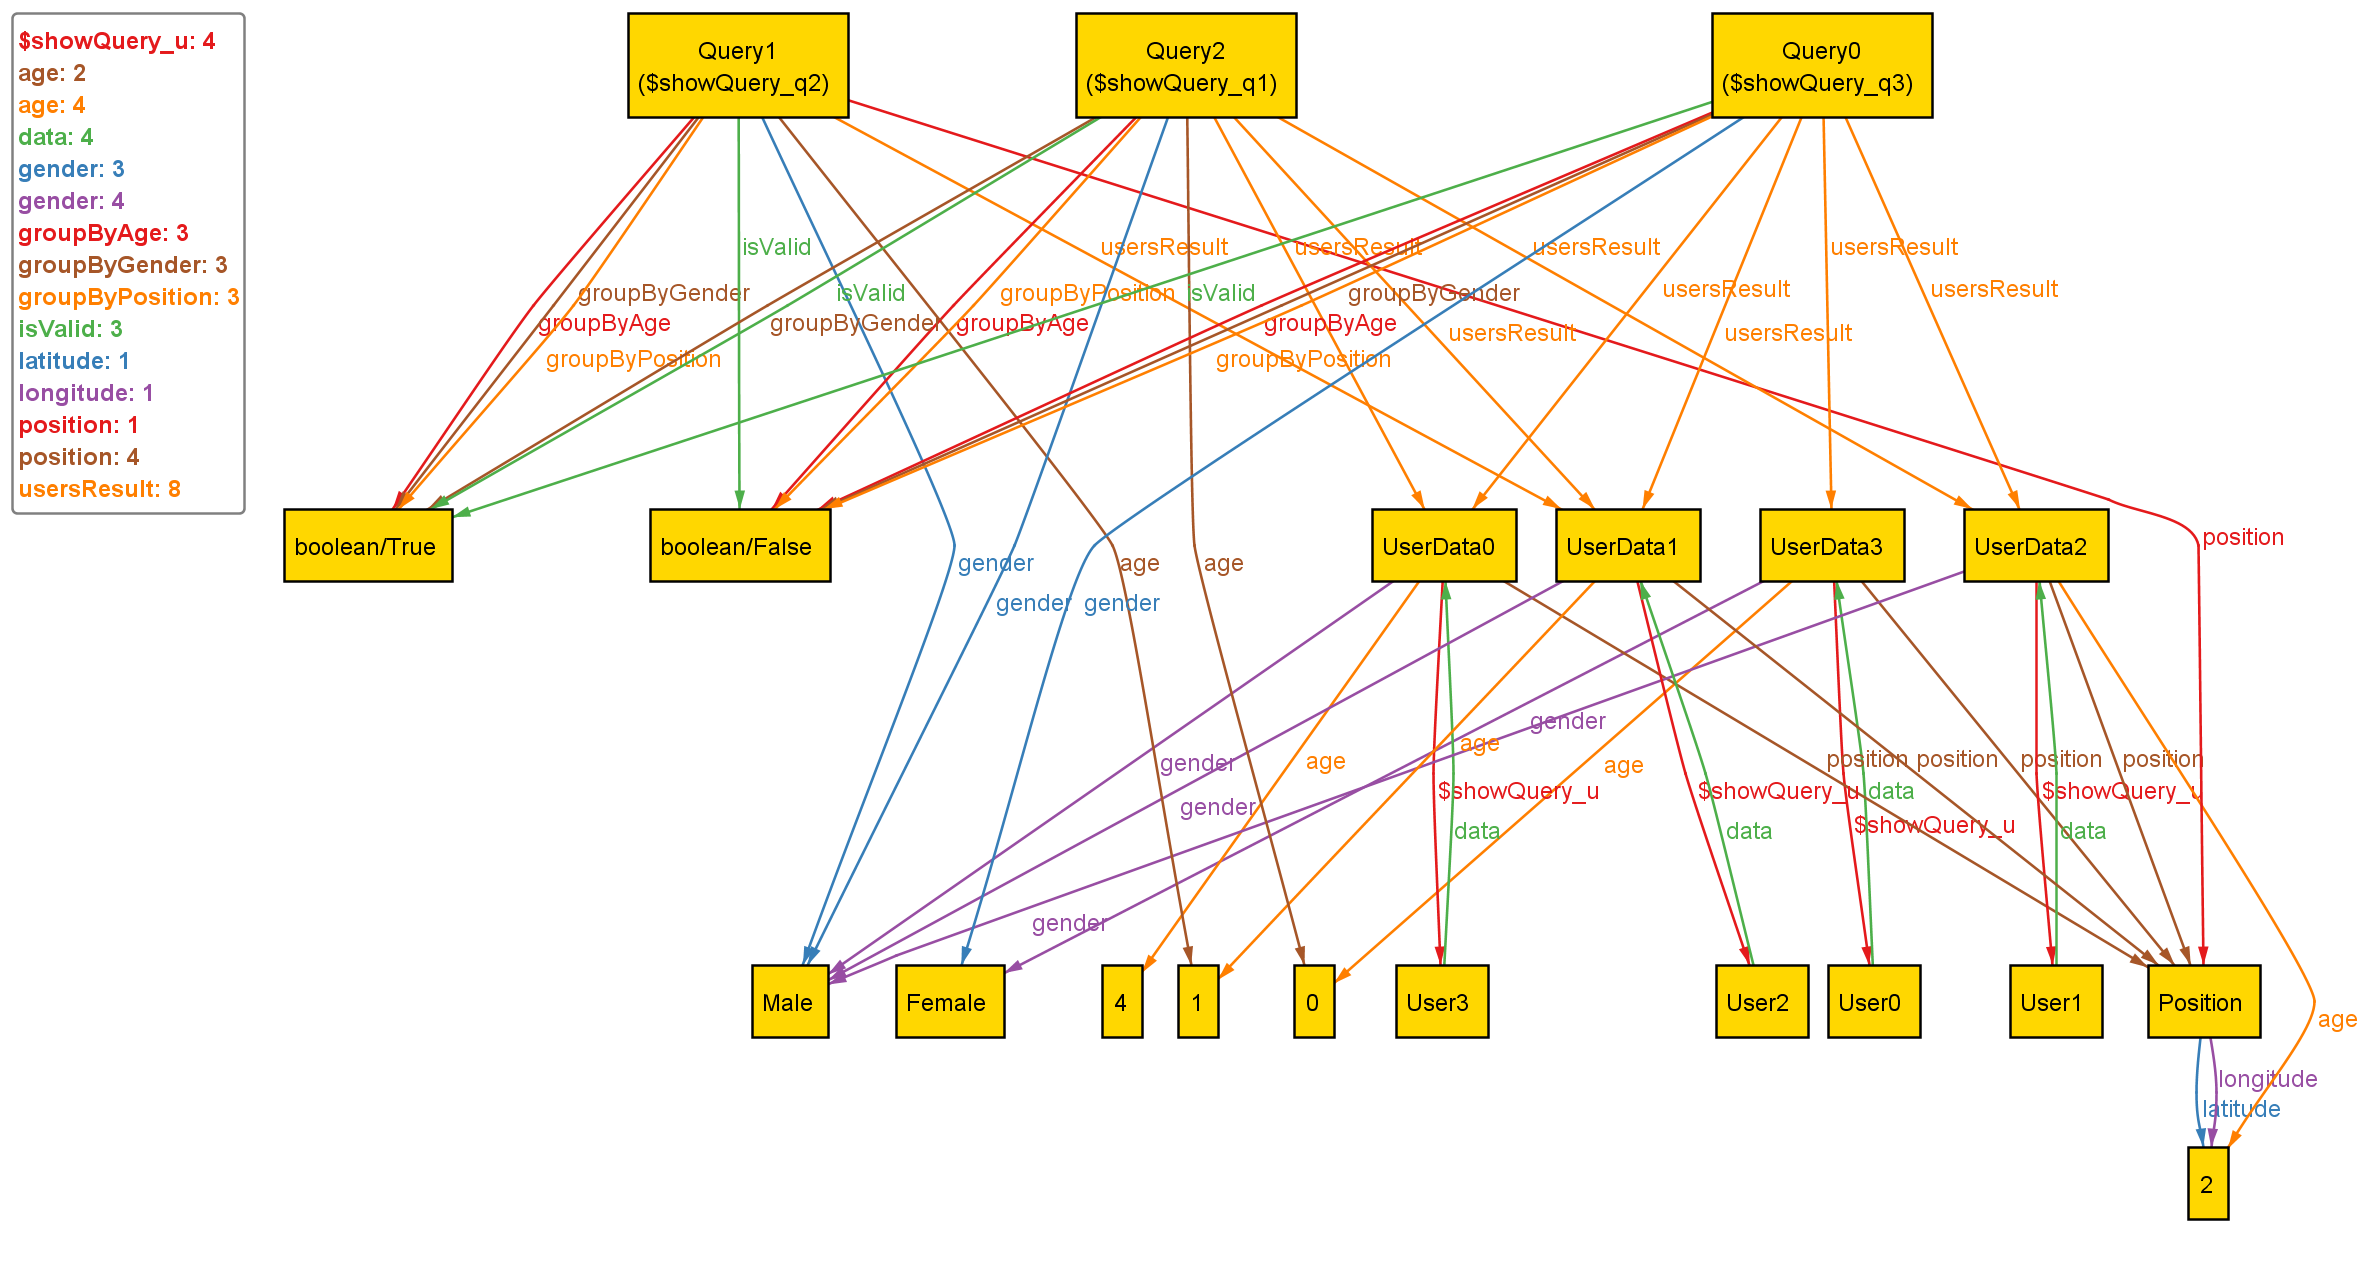
\includegraphics[height=10cm, keepaspectratio]{./Images/Alloy/data4help_1.png}
\centering
\caption{Data4Help case 1: q1 is a valid query, q2 is a non-valid query, q3 is a global query}
\end{figure}
\begin{figure}[H]
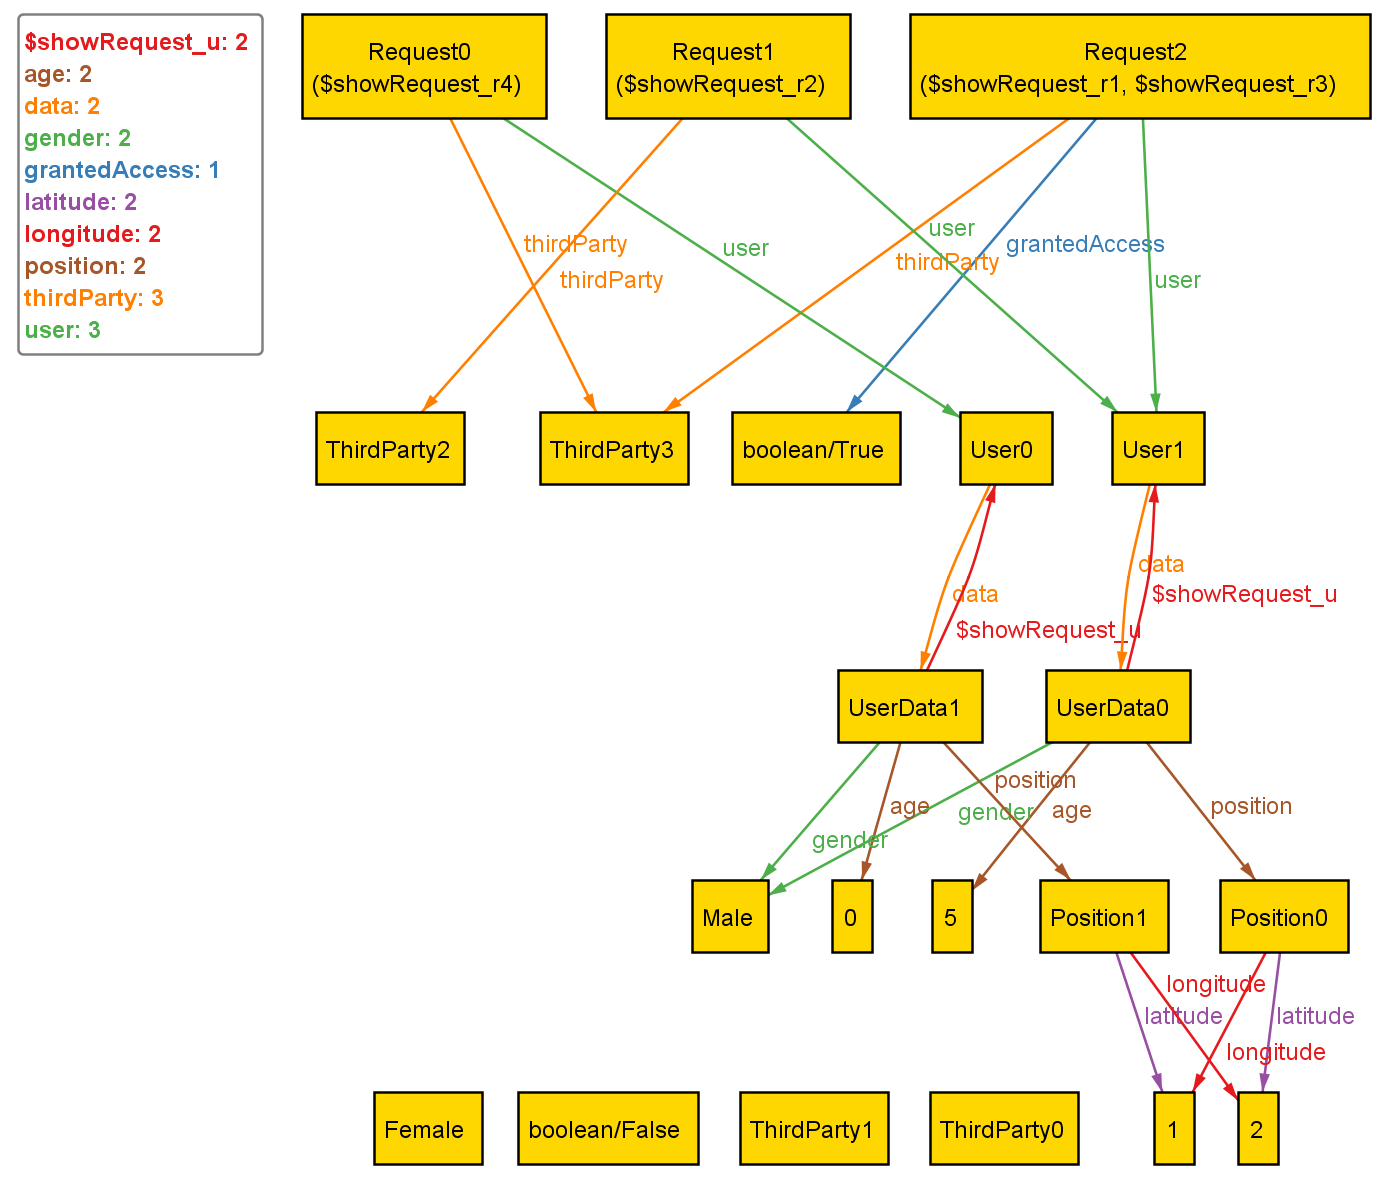
\includegraphics[width=\linewidth, height = 9cm, keepaspectratio]{./Images/Alloy/data4help_2.png}
\centering
\caption{Data4Help case 2: r1 and r2 are requests with same user, but 1 is accepted and the other is not. r3 and r4 are requests made by the same TP, one accepted and the other not}
\end{figure}

\newpage
{\color{secblue}\subsubsection{AutomatedSOS}}
\begin{figure}[H]
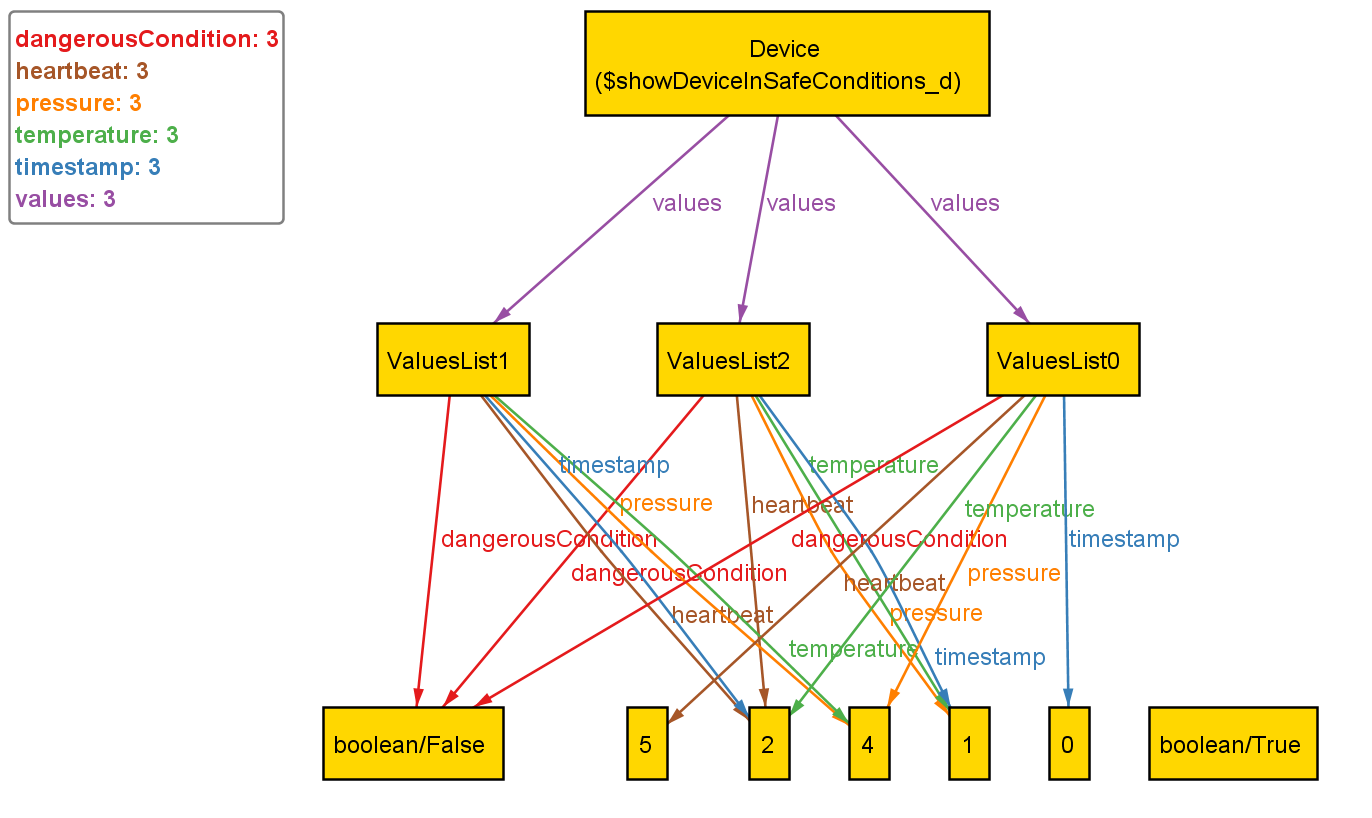
\includegraphics[width=\linewidth]{./Images/Alloy/automatedSOS_1.png}
\centering
\caption{Automated SOS case 1: a device which never registers dangerous conditions}
\end{figure}
\begin{figure}[H]
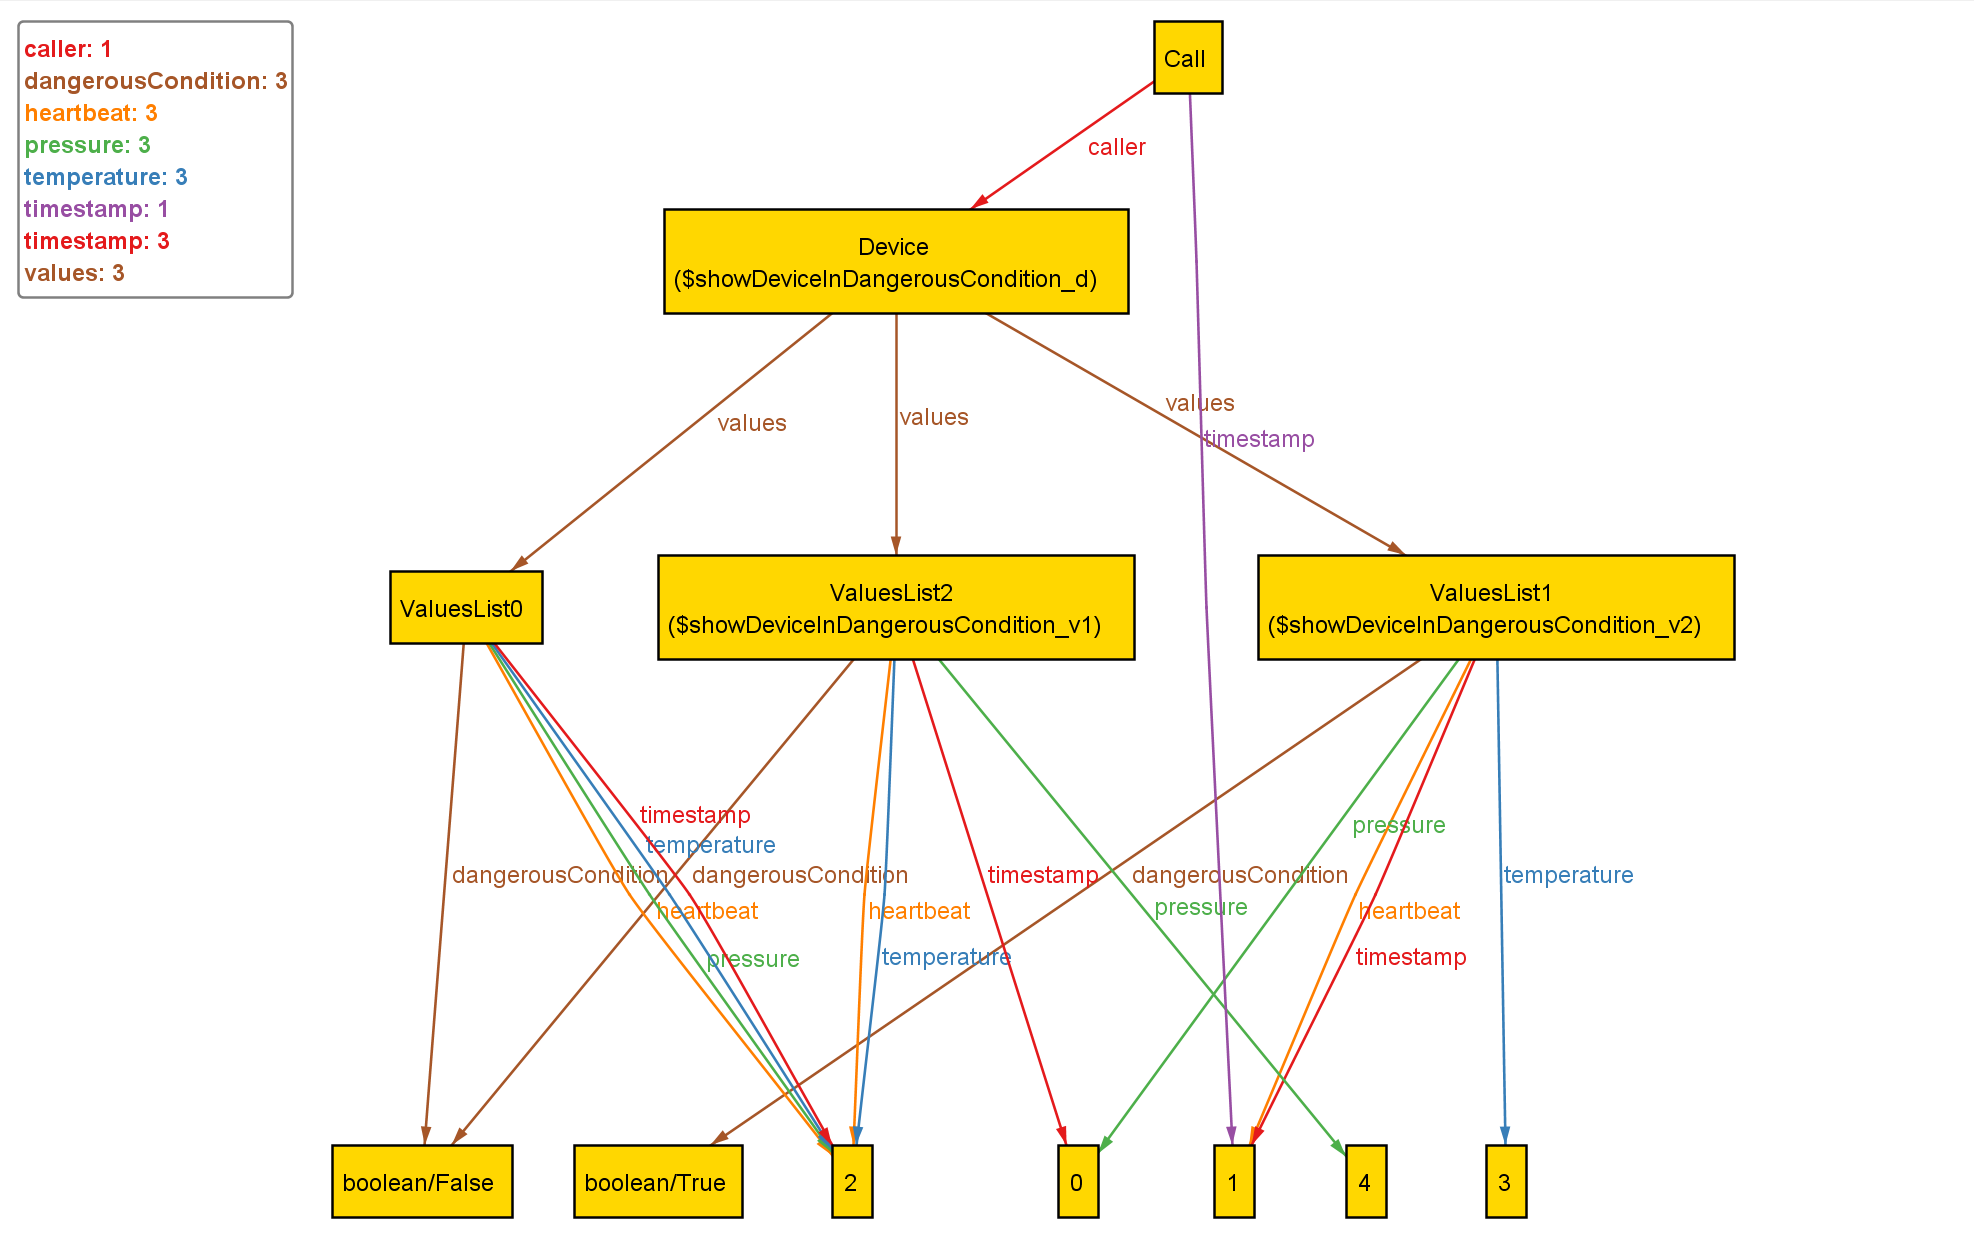
\includegraphics[width=\linewidth]{./Images/Alloy/automatedSOS_2.png}
\centering
\caption{Automated SOS case 2: a device which registers a dangerous condition starting from timestamp 1, having so a call at the same timestamp}
\end{figure}

\newpage
{\color{secblue}\subsubsection{Track4Run}}
\begin{figure}[H]
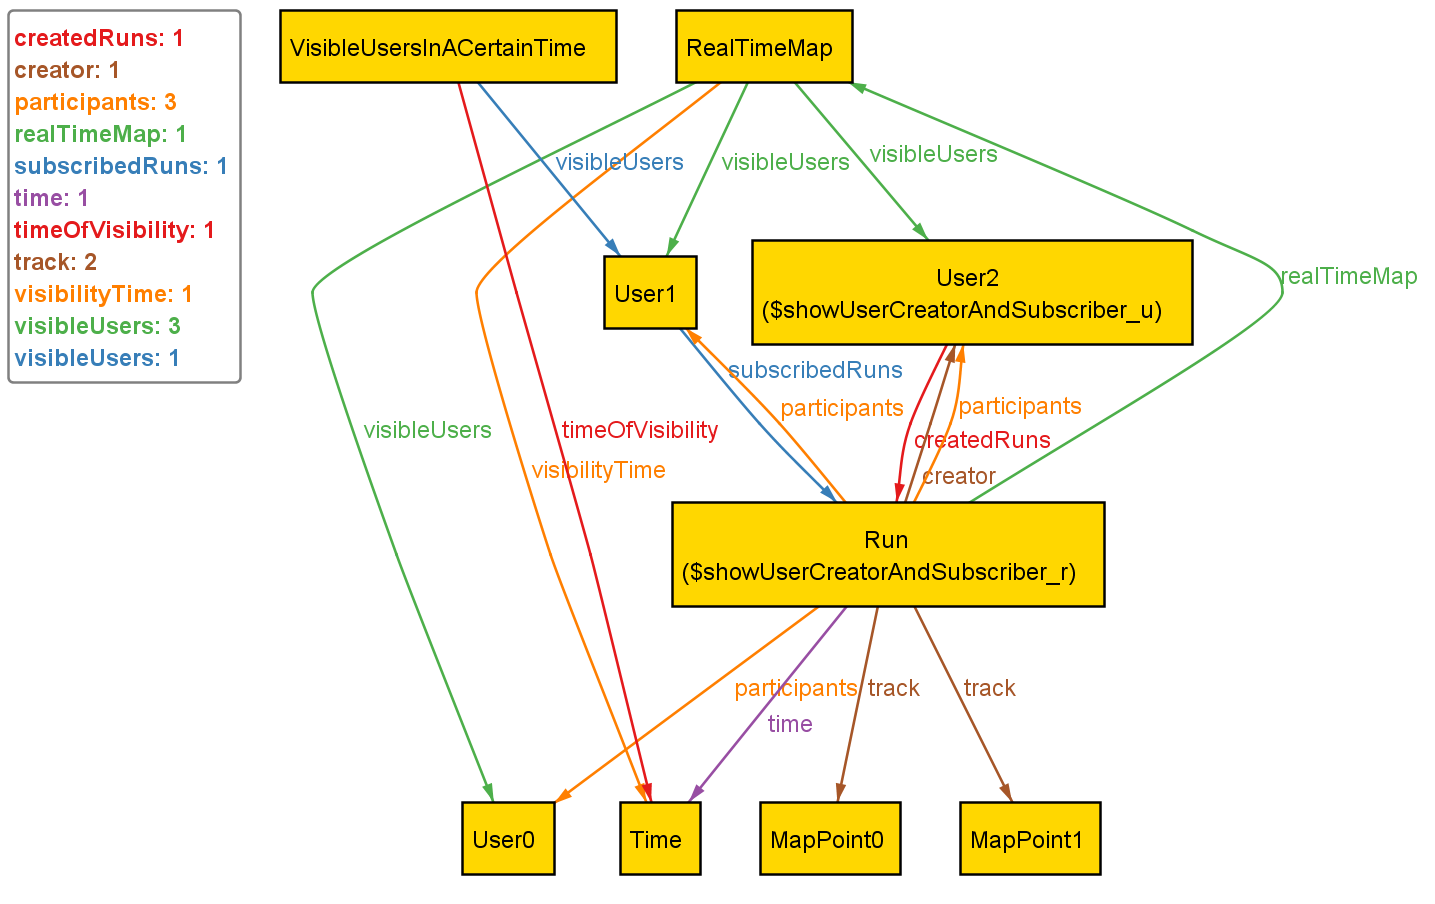
\includegraphics[width=\linewidth, height=8cm, keepaspectratio]{./Images/Alloy/track4run_v2_1.png}
\centering
\caption{Track4Run case 1: user u (User2) is at the same time the creator and a participant in the same run}
\end{figure}

\begin{figure}[H]
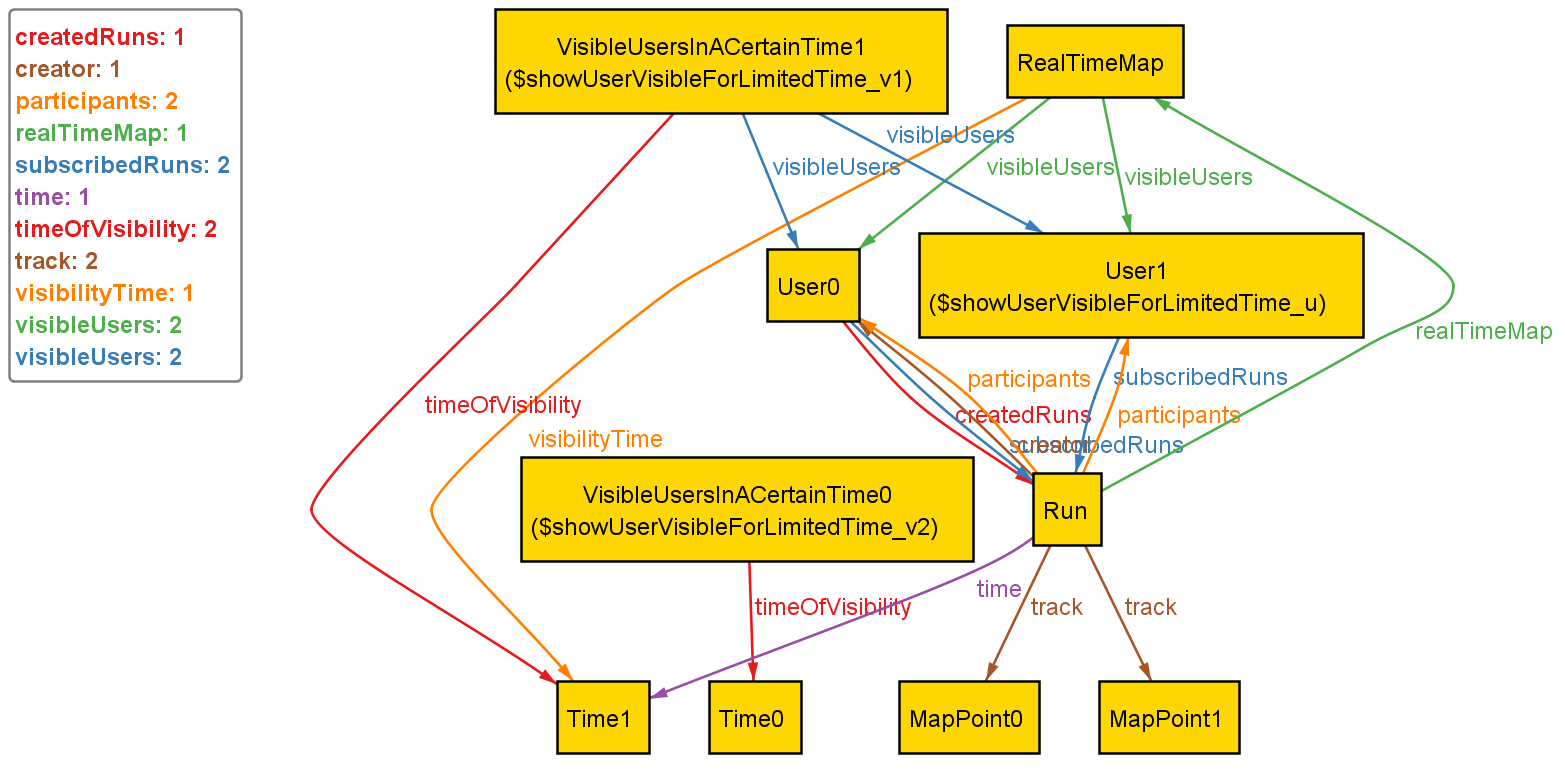
\includegraphics[width=\linewidth, height=10cm, keepaspectratio]{./Images/Alloy/track4run_v2_2.png}
\centering
\caption{Track4Run case 2: user u (User1) is visible in a certain time (Time1) but not in another (Time 0)}
\end{figure}
\newpage
{\color{secblue}\subsection{Alloy results}}
\begin{figure}[H]
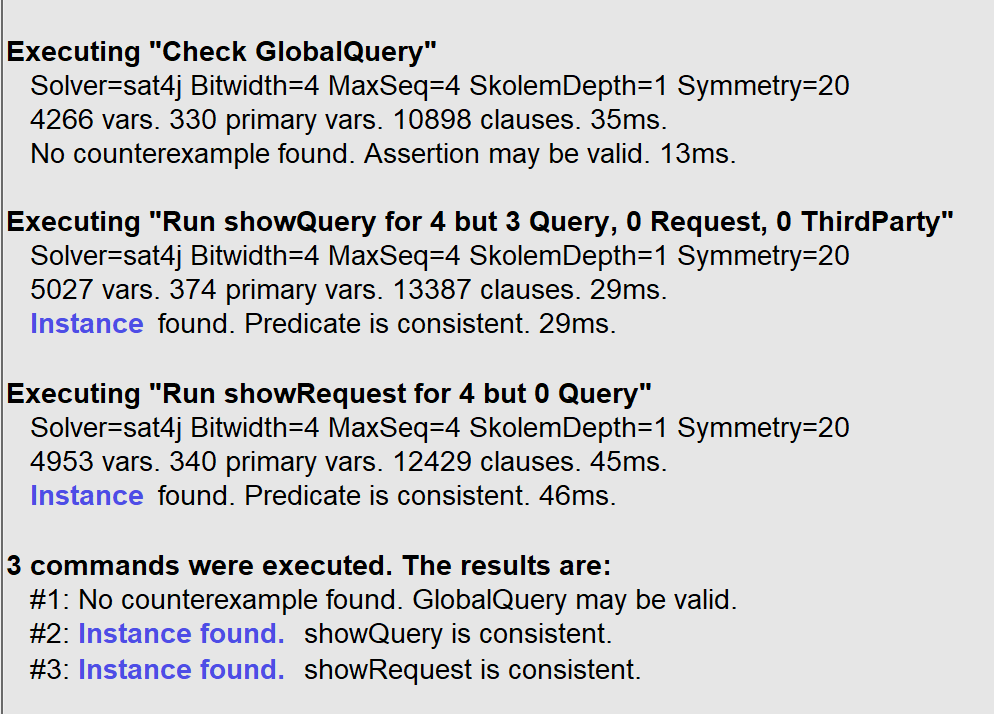
\includegraphics[width=\linewidth, height=6cm, keepaspectratio]{./Images/Alloy/data4help_results.png}
\centering
\caption{Data4Help's alloy results}
\end{figure}

\begin{figure}[H]
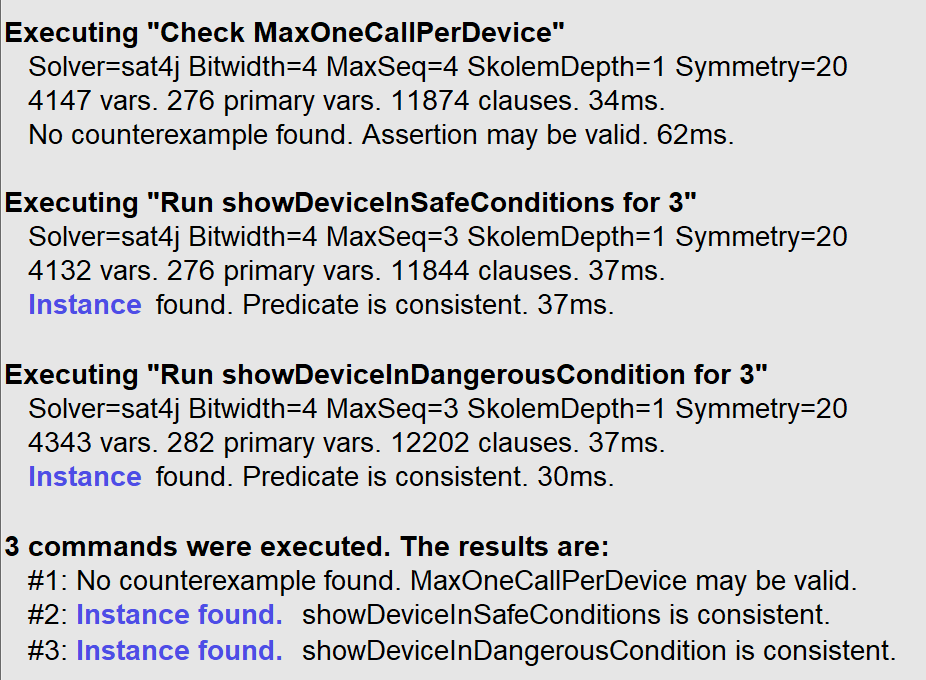
\includegraphics[width=\linewidth, height=6cm, keepaspectratio]{./Images/Alloy/automatedSOS_results.png}
\centering
\caption{AutomatedSOS' alloy results}
\end{figure}

\begin{figure}[H]
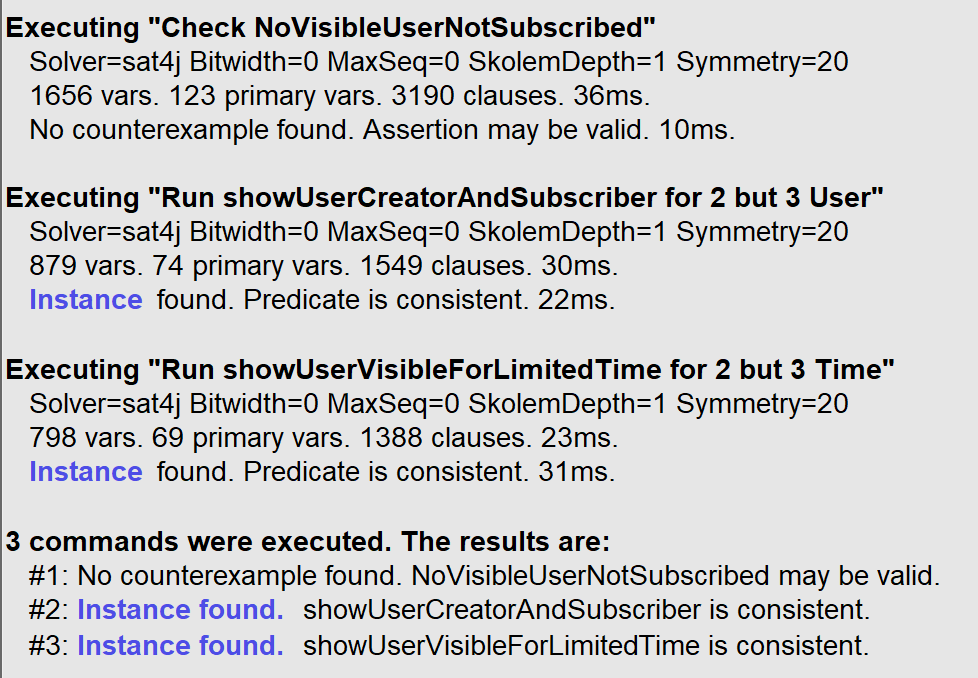
\includegraphics[width=\linewidth, height=6cm, keepaspectratio]{./Images/Alloy/track4run_v2_results.png}
\centering
\caption{Track4Run's alloy results}
\end{figure}

%------------------------------------------------------------------------------------------------------------------------------------------------
\clearpage
{\color{secblue}{\section{Effort Spent}}}
\label{sect:effort}

\subsection{Leonardo Barilani}
\begin{table}[H]
\begin{tabular}{ll}
\hline
\multicolumn{1}{|l|}{Description of the task} & \multicolumn{1}{l|}{Hours} \\ \hline
\multicolumn{1}{|l|}{Introduction}            & \multicolumn{1}{l|}{4}     \\ \hline
\multicolumn{1}{|l|}{Overall description}     & \multicolumn{1}{l|}{6}     \\ \hline
\multicolumn{1}{|l|}{Specific requirements}   & \multicolumn{1}{l|}{14}     \\ \hline
\multicolumn{1}{|l|}{Formal analysis using Alloy}   & \multicolumn{1}{l|}{2}   \\ \hline
\end{tabular}
\end{table}


\subsection{William Bonvini}
\begin{table}[H]
\begin{tabular}{ll}
\hline
\multicolumn{1}{|l|}{Description of the task} & \multicolumn{1}{l|}{Hours} \\ \hline
\multicolumn{1}{|l|}{Introduction}            & \multicolumn{1}{l|}{4}     \\ \hline
\multicolumn{1}{|l|}{Overall description}     & \multicolumn{1}{l|}{4}     \\ \hline
\multicolumn{1}{|l|}{Specific requirements}   & \multicolumn{1}{l|}{22}     \\ \hline
\multicolumn{1}{|l|}{Formal analysis using Alloy}   & \multicolumn{1}{l|}{2}   \\ \hline
\end{tabular}
\end{table}


\subsection{Lorenzo Carnaghi}
\begin{table}[H]
\begin{tabular}{ll}
\hline
\multicolumn{1}{|l|}{Description of the task} & \multicolumn{1}{l|}{Hours} \\ \hline
\multicolumn{1}{|l|}{Introduction}            & \multicolumn{1}{l|}{4}     \\ \hline
\multicolumn{1}{|l|}{Overall description}     & \multicolumn{1}{l|}{4}     \\ \hline
\multicolumn{1}{|l|}{Specific requirements}   & \multicolumn{1}{l|}{4}     \\ \hline
\multicolumn{1}{|l|}{Formal analysis using Alloy}   & \multicolumn{1}{l|}{16}   \\ \hline
\end{tabular}
\end{table}


%------------------------------------------------------------------------------------------------------------------------------------------------
\clearpage
\addcontentsline{toc}{section}{References}
\bibliographystyle{plain}
\bibliography{main}
%------------------------------------------------------------------------------------------------------------------------------------------------




\end{document}
